\chapter{\texorpdfstring{\ds\ and \dpl\ reconstruction strategy in proton-proton collisions}{Ds+ and D+ reconstruction strategy in proton-proton collisions}}\label{chap:reconstruction}

\begin{sloppypar}
Due to their mean proper decay lengths (\ct) of \SI{151.2}{\micro\meter} and \SI{309.8}{\micro\meter} respectively~\cite{pdg}, \ds\ and \dpl\ mesons and their charge conjugates cannot be directly detected, as they typically decay before reaching the ALICE detector. Consequently, their production is measured through the reconstruction of their decay products. This analysis exploits their hadronic decays into $\ds (\dpl) \rightarrow \mathrm{\phi\pi^+ \rightarrow K^+K^-\pi^+}$ and their charge conjugates, with a branching ratio of $(2.21\pm0.06)\times10^{-2}$ \mbox{$\left((2.69^{+0.07}_{-0.08})\times10^{-3}\right)$}~\cite{pdg}, respecitvely. An additional hadronic decay channel of the \dpl meson with a larger BR of \mbox{$(9.38\pm0.16)\times10^{-2}$}~\cite{pdg} could be exploited~\cite{ALICE:2017olh}. However, the reconstruction of the two D-mesons species in the same decay channel allows for the cancellation of many of the systematic uncertainties affecting the measurement, potentially leading to a more precise \ds/\dpl production yield ratio measurement. The choice of reconstructing D mesons through their decays into a hadronic final state allows for the full reconstruction of the decay topology, therefore providing access to the D-meson kinematics and the reconstruction of the secondary vertex, which is used in the selection of the signal against the large combinatorial background. Semileptonic decay measurements are in fact affected by larger uncertainties due to the presence of neutrinos in the final state, which are not detected. In addition, the decay into the resonant $\phi(1020)$ state opens up the possibility of exploiting the invariant mass of the $\phi$ meson for the selection of the D-meson candidates. A sketch of the decay topology of \ds and \dpl mesons into $\mathrm{\phi\pi^+ \rightarrow K^+K^-\pi^+}$ is shown in Fig.~\ref{fig:DecaySketch}.
\end{sloppypar}

\begin{figure}[htb]
    \centering
    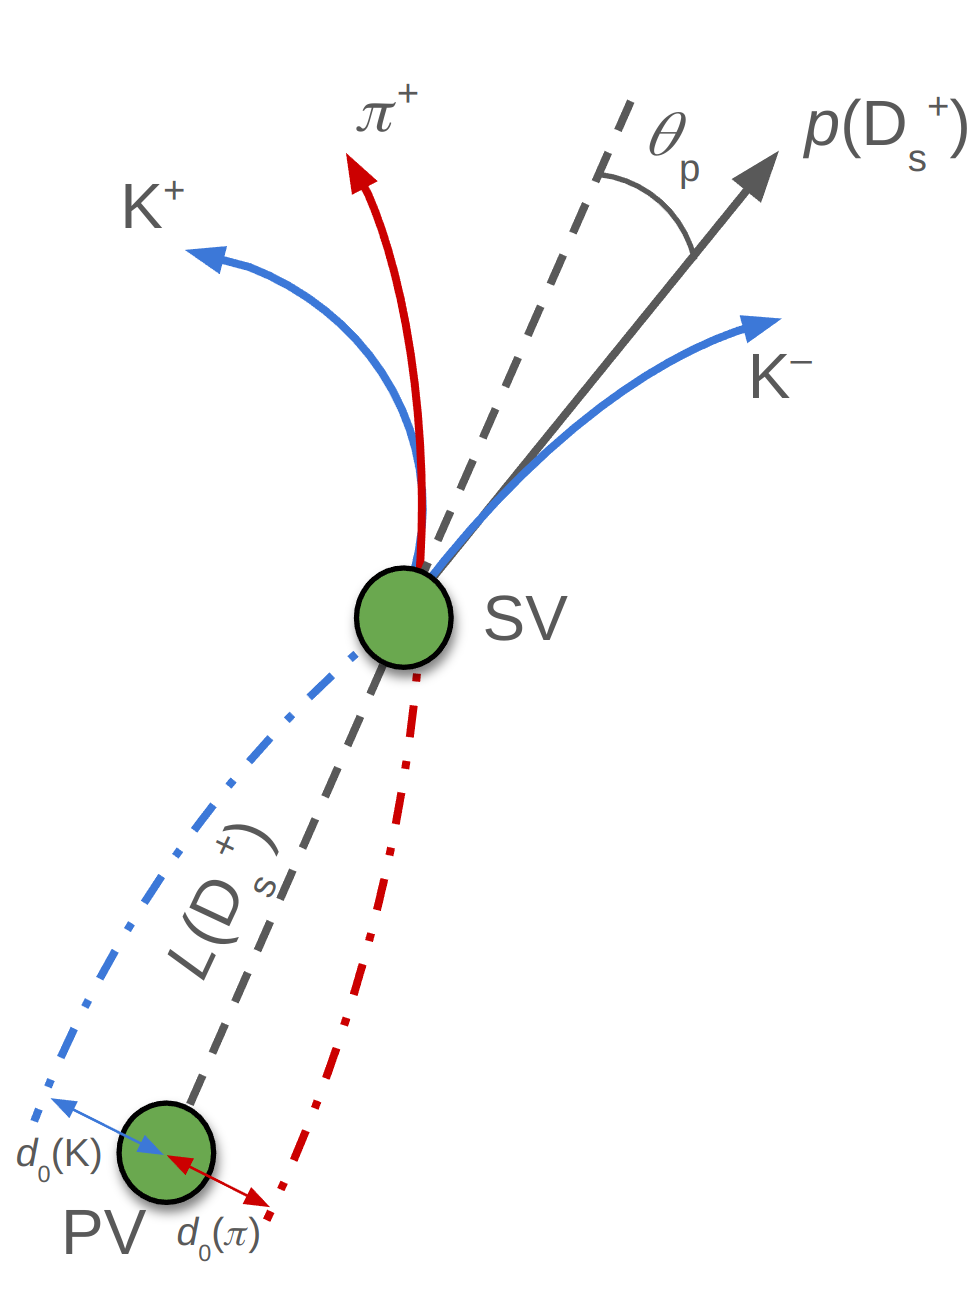
\includegraphics[width=0.48\linewidth]{Figures/Chapter 4/sketchPrompt.png}
    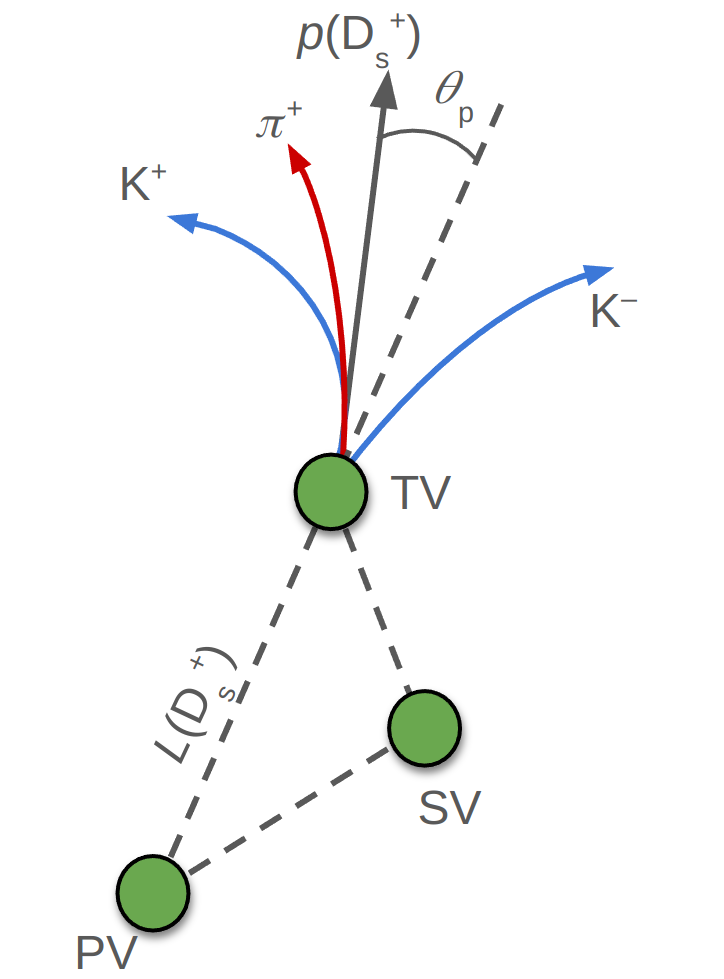
\includegraphics[width=0.48\linewidth]{Figures/Chapter 4/sketchNonPrompt.png}
    \caption{Sketch of the decay topology of \ds and \dpl mesons into $\mathrm{\phi\pi^+ \rightarrow K^+K^-\pi^+}$ for prompt (left) and non-prompt (right) \ds meson.}
    \label{fig:DecaySketch}
\end{figure}

\ds\ and \dpl\ mesons (and their charge conjugates) are reconstructed in three different steps: i) firstly, charged tracks are reconstructed at midrapidity ($\lvert\eta\rvert < 0.8$) exploiting the information of the ITS and TPC detectors; ii) \ds\ and \dpl\ candidates are constructed by combining triplets of tracks with the appropriate charge signs, i.e., (+, --, +) for \ds\ and \dpl\ mesons, and (--, +, --) for their antiparticles; iii) lastly, the \ds\ and \dpl\ candidates are selected by applying a set of topological, kinematical, and Particle-IDentification (PID) selections. Given the large number of tracks produced in a pp collision and the comparatively small production cross-section of charmed hadrons as well as the small BRs of the considered decay modes, the vast majority of the constructed \ds\ and \dpl\ candidates are obtained from the combination of uncorrelated tracks, which do not originate from the decay of a \ds (\dpl) meson. This results in a large \emph{combinatorial background}, which has to be suppressed in order to extract the signal of the D mesons. 

The spatial resolution capabilities of the ALICE detector described in Chapter~\ref{chap:ALICE} enable the separation of the secondary decay vertices of D mesons from the primary interaction vertex, which consents the development of an analysis based on the reconstruction and selection of secondary-vertex topologies characterised by relatively large separations from the primary interaction vertex. Furthermore, the PID of the decay products can be further exploited to improve the selection of D mesons.

Two distinct categories of D mesons emerge based on their production mechanism: \emph{prompt}, directly produced in the hadronisation of a charm quark or through the strong decay of a directly produced excited charm-hadron or charmonium state, and \emph{non-prompt} (also referred to as \emph{feed-down}), produced in the decay of a hadron containing a beauty quark. Decay vertices of feed-down D mesons are on average more displaced from the primary interaction point with respect to promptly-produced ones, due to the larger mean proper decay length of beauty hadrons (\ct $\sim$ 500 µm~\cite{pdg}) as compared to charm hadrons. Therefore, by exploiting selection criteria based on displaced decay-vertex topologies, it is possible not only to separate D-meson signals from the combinatorial background, but also to discriminate between feed-down and prompt D mesons.

\section{Data sample and event selection}
The analysis reported in this Thesis is performed on a dataset of pp collisions at a centre-of-mass energy of \thirteen, collected by the ALICE detector during the 2022 data-taking period. The data sample is collected using a Minimum-Bias trigger (the \code{Sel8} trigger), which selects events that satisfy the requirement of having a signal coincidence in the FT0-A and FT0-C detectors. Furthermore, since it is observed that the readout of the TPC (which is performed at the end of each time frame (TF)) causes a drop in the track reconstruction efficiency, it was decided to exclude the collisions read out during this time interval (\emph{TF border} selection). An additional requirement is imposed on the primary vertex position along the beam axis, $\lvert z_{\mathrm{vtx}}\rvert<10$~cm, to ensure that the point where protons have collided is located within the region of the detector where the tracking efficiency is optimal. Of the total 59.2 billion collected events, only 54.7 billion have been analysed, corresponding to an integrated luminosity of $\mathcal{L}_\mathrm{int}\sim \SI{1}{\per\pico\barn}$. Around 3\% of the events are rejected due to the minimum bias trigger, about 1\% due to the TF border selection, and 4\% of the events are rejected due to the requirement on the $z_{\mathrm{vtx}}$ position. A summary of the event selection is shown in Fig.~\ref{fig:EvSel}.


\begin{figure}[htb]
    \centering
    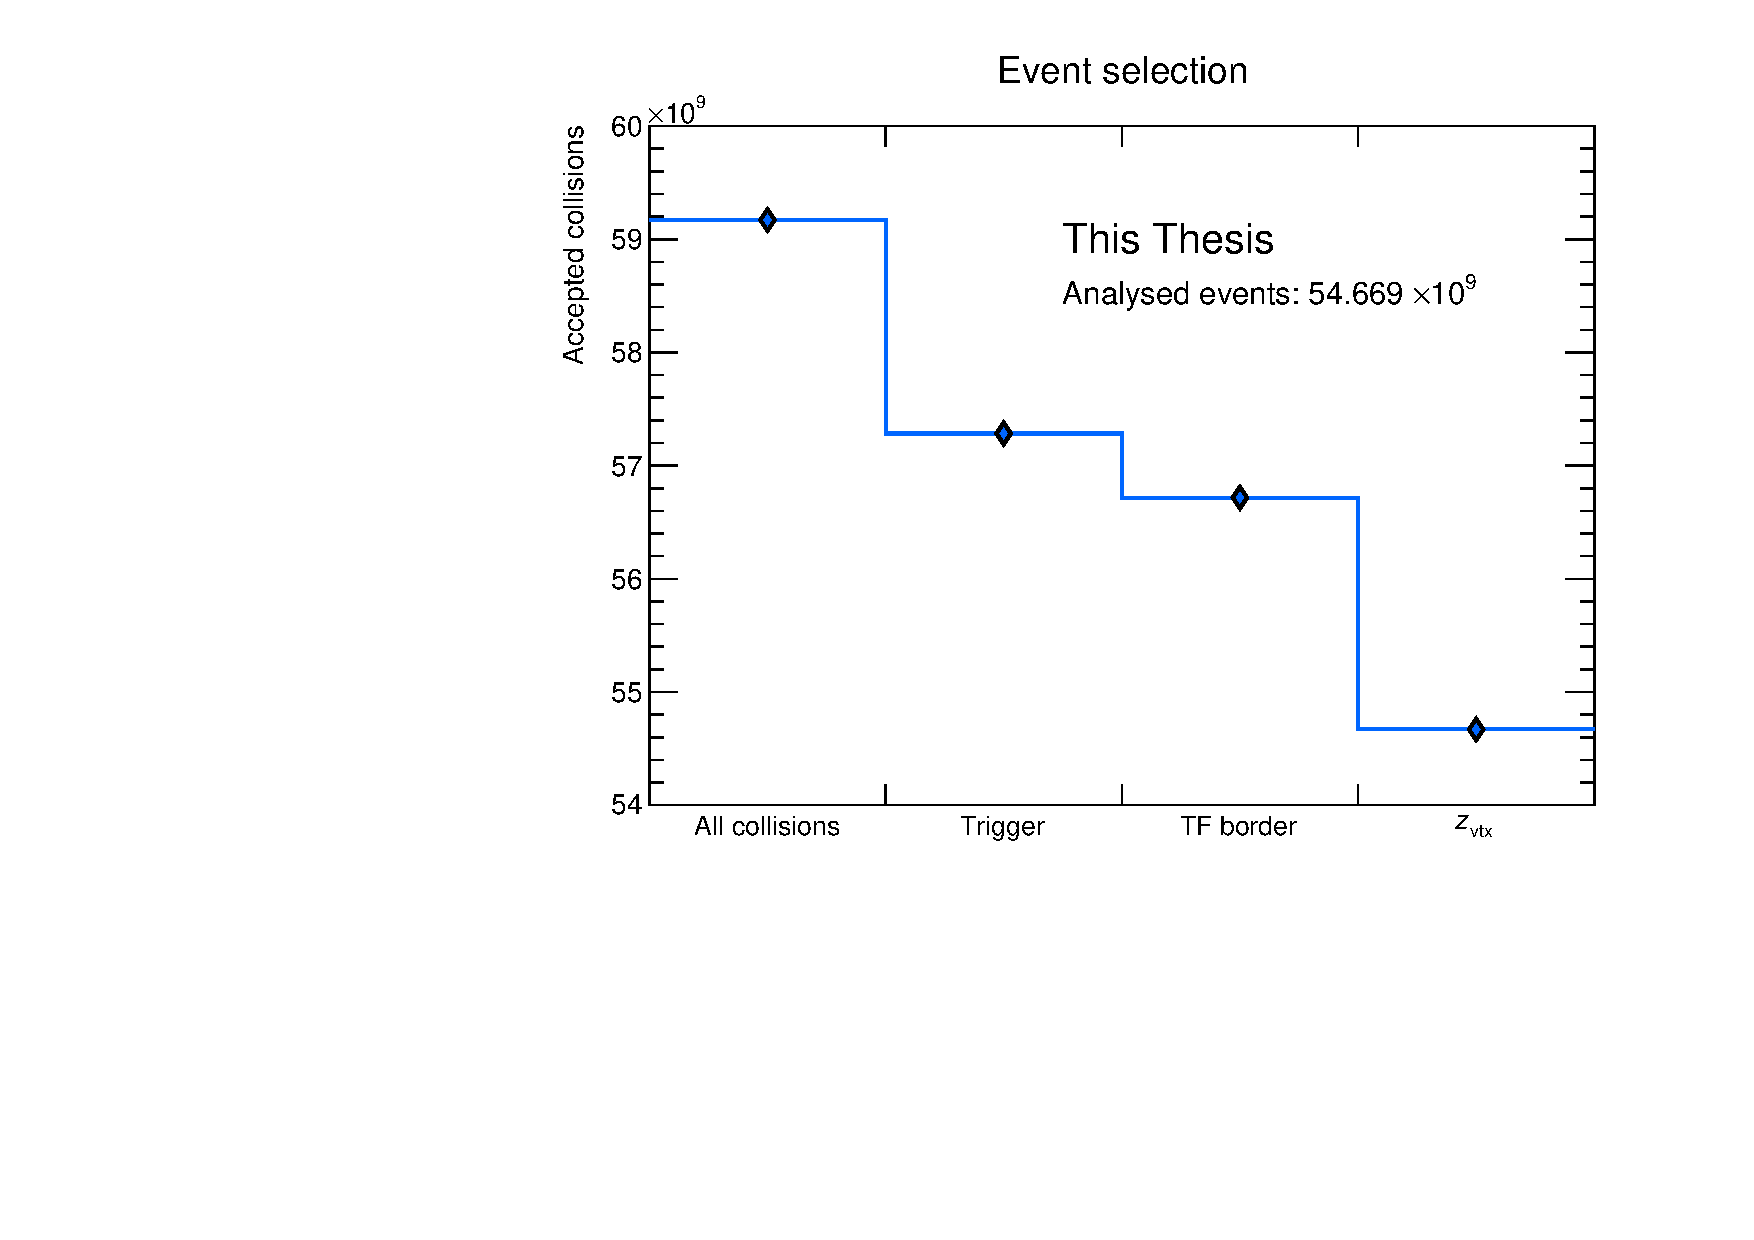
\includegraphics[width=0.7\linewidth]{Figures/Chapter 4/EventSelection.pdf}
    \caption{Summary of the event selection criteria applied to the data sample.}
    \label{fig:EvSel}
\end{figure}

\section{\texorpdfstring{\ds and \dpl reconstruction workflow}{Ds+ and D+ reconstruction workflow}}
\begin{figure}
    \centering
    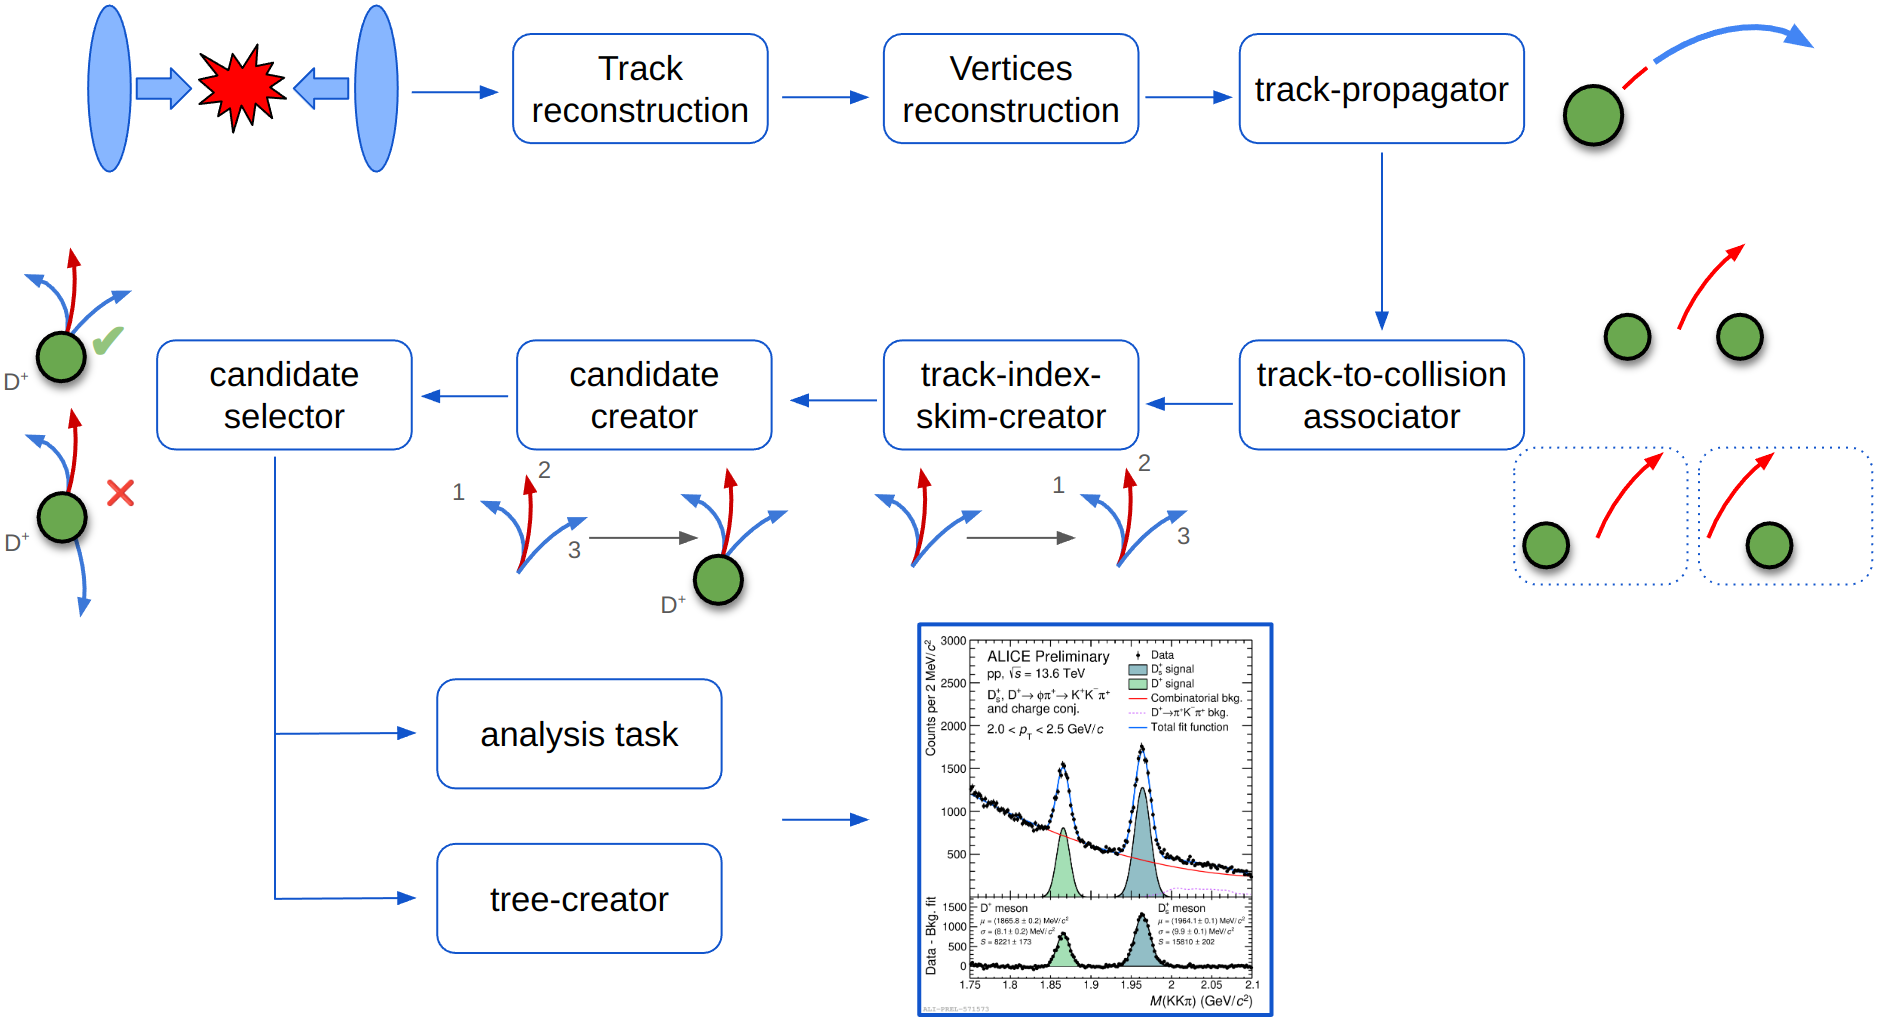
\includegraphics[width=\linewidth]{Figures/Chapter 4/Workflow_Scheme.png}
    \caption{Schematic representation of the reconstruction workflow of \ds and \dpl mesons.}
    \label{fig:RecoWorkflow}
\end{figure}
The reconstruction of \ds and \dpl mesons is a complex process performed in many subsequent steps. As stated in Chapter~\ref{chap:ALICE}, the reconstructed data are stored in AOD format. This format contains essential information about the reconstructed tracks, which are parameterised at the innermost update point, i.e., the closest point to the primary vertex with a detected track signal. Since the track parametrisation is not the same for each track, as missing hits in the ITS can lead to different radii of the innermost update points, the tracks are propagated to the point of closest approach to the primary vertex, and their parameters are updated accordingly. This procedure is performed in the \code{track-propagator} workflow, and only tracks passing a set of predefined quality requirements are selected. 

Because of the continuous readout, there exists the possibility that a single track is found to be compatible with multiple collisions (these tracks are named \emph{ambiguous tracks}). In the AOD files, the ambiguous tracks are only associated with the first space-time-compatible collision. In order to increase the reconstruction efficiency, the \code{track-to-collision associator} workflow associates each track with all compatible collisions\textcolor{red}{cosa vuol dire compatibili? commento prino}. This process significantly increases the reconstruction efficiency of decaying particles.

For each considered collision, combinations of two or three tracks are built in the \code{track-index-skim-creator} workflow, producing candidates of charmed hadrons, in particular for the hadronic decays of $\dz\rightarrow\mathrm{K^-\pi^+}$, $\mathrm{D^{*+}}\rightarrow\mathrm{D^0\pi^+}$, $\dpl\rightarrow\pi^+\mathrm{K^-}\pi^+$, \mbox{$\ds(\dpl)\rightarrow\mathrm{K^+K^-\pi^+}$}, $\lc\rightarrow\mathrm{pK^-\pi^+}$, and $\mathrm{\Xi_c^+}\rightarrow\mathrm{pK^-\pi^+}$. The workflow produces a table of track indices for the combinations passing a set of loose selection criteria, which depends on the considered hadron species. Candidates for each particle species and their decay vertices are created in the \code{candidate-creator} workflow starting from the track indices of combinations saved by the \code{track-index-skim-creator}, and those passing the more stringent analysis selection criteria are flagged in the \code{candidate-selector} workflow. The \code{tree-creator} (\code{analysis-task}) workflow produces the final output of the analysis, which consists of a ROOT tree (several ROOT histograms) containing the properties of selected candidates.

\section{Vertex reconstruction and D-meson selection}

The track and primary vertex reconstruction is performed both in the ``syncronous'' reconstruction, performed quasi-online for quality-control and detector-calibration purposes, and in the ``asynchronous'' reconstruction performed on the stored raw data a few days after the data taking and after the detector calibrations have been performed offline, using information from the central barrel detectors. Firstly, the hits recorded in the ITS and TPC detectors are converted into \emph{clusters}, corresponding to groups of hits produced by a single particle interacting with a detector element. They contain information about position, signal, timing, and the corresponding uncertainties. Then, a first estimation of the interaction-vertex position is obtained by using clusters in the ITS inner barrel. Track segments, called tracklets, are constructed by associating pairs of clusters from different layers within a predefined azimuthal acceptance window. The primary vertex is obtained as the point in space where the largest number of tracklets converge. 

Tracks are constructed using ITS~\cite{Concas:2878385} and TPC~\cite{Rohr:2018cxc} standalone reconstructions using a Kalman filter-based algorithm~\cite{Fruhwirth:1987fm}. Track information in the two detectors is then matched within compatible time windows (ITS-TPC matching) to build the \emph{global} tracks. These are subsequently refitted in the outward direction and matched to outer detectors, e.g., TRD, TOF, and HMPID~\cite{Rohr:2019ava}. The propagation to detectors located beyond the TPC radius does not update the kinematic track parameters, but it is used to attach to the track the information needed for particle identification. Tracks are then re-fitted towards the interaction point using the previously found clusters, and the final track parameters and covariance matrix are computed and stored at the innermost hit. The primary vertex is then determined using the tracks reconstructed in the previous steps.
The decay vertex of the candidate is reconstructed through a minimisation of a $\chi^2$-like quantity, denoted as $D$:
\begin{equation*}
    D = \sqrt{\sum_{i=1}^3 \left[\left(\frac{x_i-x_0}{\sigma_{x_i}}\right)^2 + \left(\frac{y_i-y_0}{\sigma_{y_i}}\right)^2 +\left(\frac{z_i-z_0}{\sigma_{z_i}}\right)^2\right]}\quad ,
\end{equation*}
where ($x_i,y_i,z_i$) and ($\sigma_{x_i},\sigma_{y_i},\sigma_{z_i}$) represent the position and the uncertainty of the i-th track at the point of closest approach, respectively, while ($x_0,y_0,z_0$) denotes the position of the reconstructed vertex. The invariant mass and momentum of the \ds\ and \dpl\ candidates are computed from the energy and momentum of the measured tracks evaluated at the point of closest approach to the decay vertex. The momentum of the candidate is defined as the sum of the momenta of the three tracks. For the invariant mass computation, the kaon mass is always assigned to the track with opposite charge sign with respect to the D-meson candidate (\emph{opposite-sign track}). For the two \emph{like-sign tracks}, the two pion-kaon mass hypothesis combinations \big(i.e. ($\mathrm{K^+K^-\pi^+}$) and ($\mathrm{\pi^+K^-K^+}$) for positively charged candidates\big) are considered. 

The vast majority of the created \ds- and \dpl-meson candidates belong to the large combinatorial background. To increase the signal-over-background ratio and the statistical significance of the measurement, tight selections are required to suppress background candidates. The analyses presented in this Thesis exploit several selection criteria, which can be divided into:
\begin{enumerate}[i]
    \item Track-quality selections
    \item Selections based on the decay topology and kinematics
    \item Particle identification of the decay products
\end{enumerate}
In the following, the variables used to select D mesons and some of the applied selections are described in more detail.

\subsection{Track-level selections}
Only tracks that successfully pass strict quality and kinematic requirements are considered eligible for inclusion in the construction of \ds- and \dpl-meson candidates. In particular, only ITS-TPC tracks with at least 70 (out of a maximum of 159) TPC crossed rows (i.e., the total number of hit TPC pad rows) are selected. To improve the vertex reconstruction procedure, at least one hit in the 3 innermost layers of the ITS, which compose the ITS inner barrel, was required. Track-quality requirements of $\chi^2$ per TPC cluster smaller than 4 and $\chi^2$ per ITS cluster smaller than 36 have been applied.

Secondary vertices of \ds- and \dpl-meson candidates are constructed using tracks having $\lvert\eta^\mathrm{dau}\rvert < 0.8$ and $\pt^\mathrm{dau} > 0.3$~\gevc. These kinematical selections limit the rapidity acceptance of D mesons, which steeply decreases for $\lvert y\rvert > 0.5$ at low \pt and for $\lvert y\rvert > 0.8$ for $\pt \gtrsim 5~\gevc$, as shown in Fig.~\ref{fig:RapidityAcceptance}. The applied track-quality selection criteria are summarised in Table~\ref{tab:trackSel}. 
\begin{figure}[htb]
    \centering
    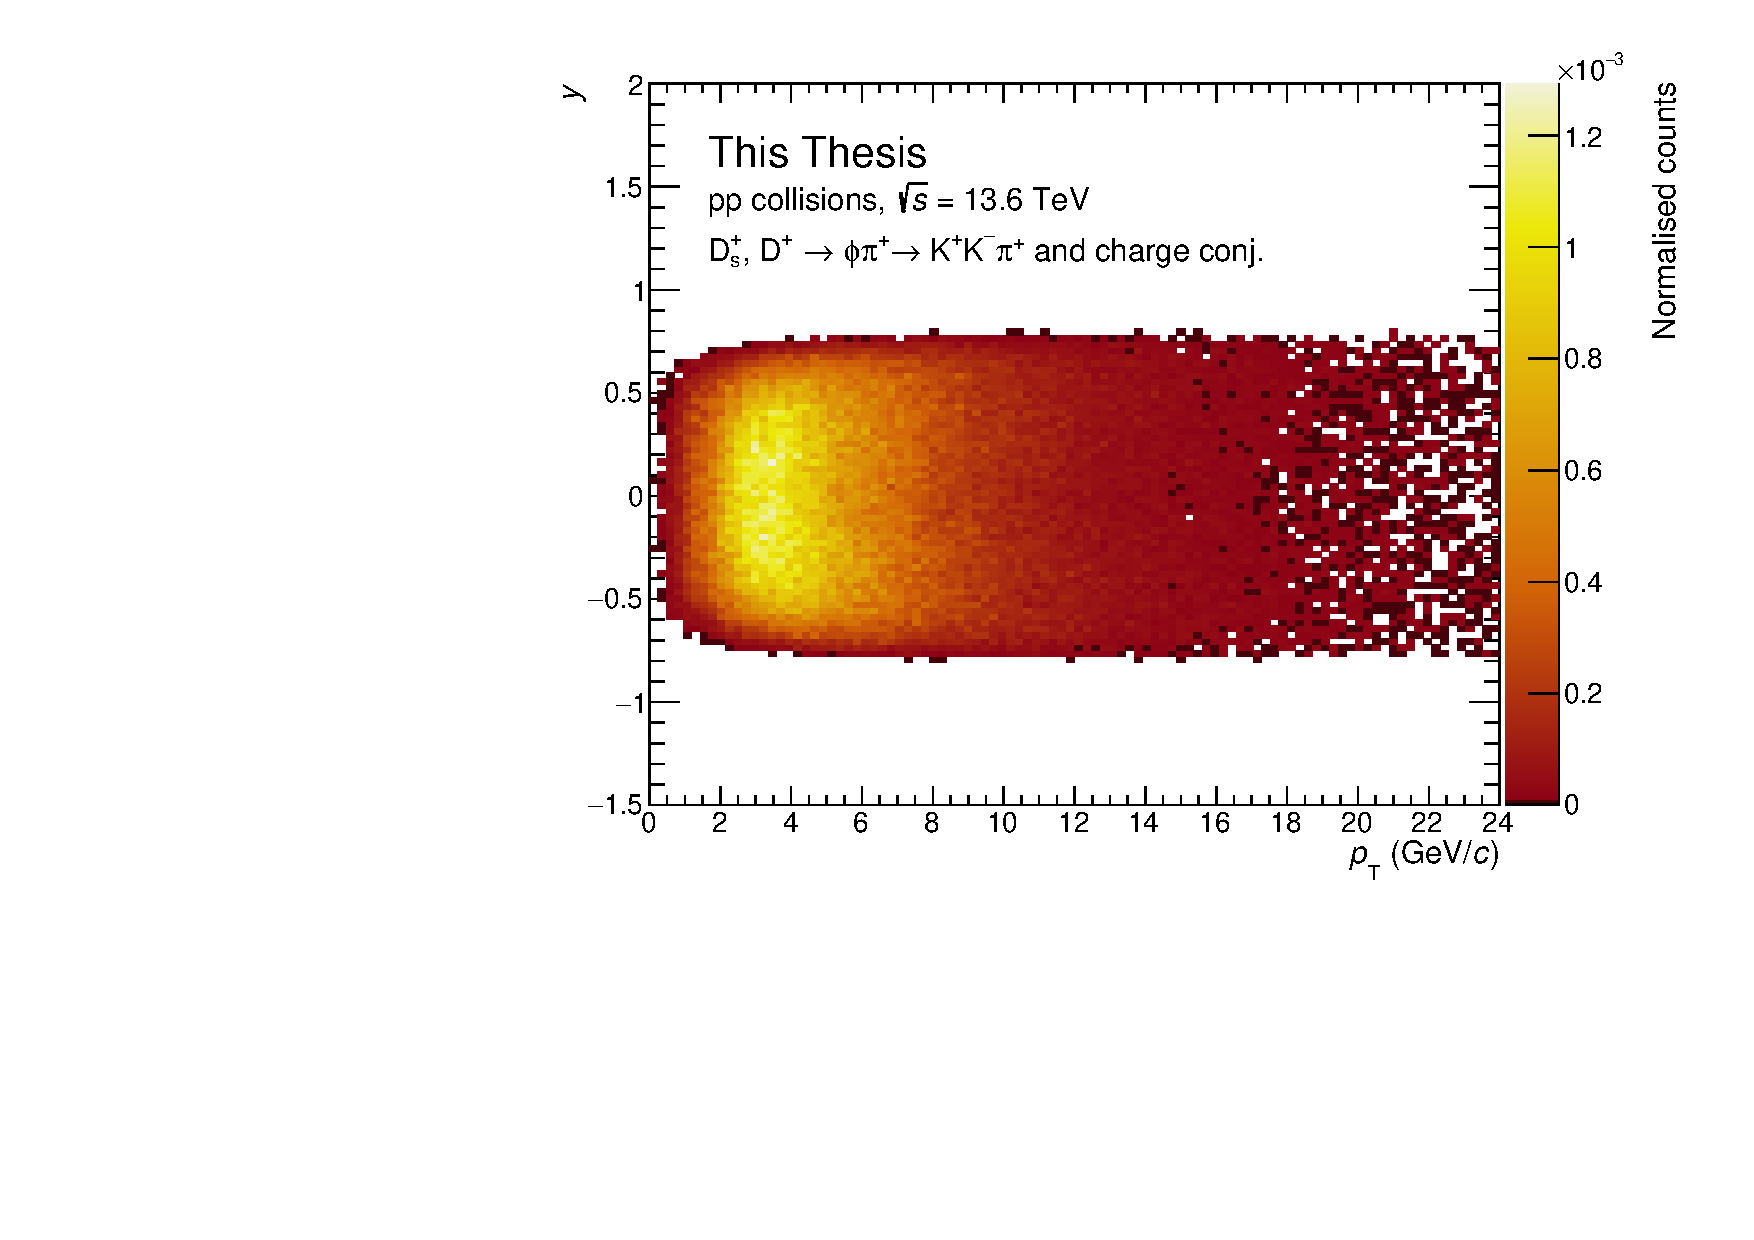
\includegraphics[width=0.7\linewidth]{Figures/Chapter 4/PtVsY.pdf}
    \caption{Rapidity and transverse momentum distribution of reconstructed \ds and \dpl mesons in pp collisions at \thirteen. The kinematical selections applied on the daughter tracks, requiring $\lvert\eta^\mathrm{dau}\rvert < 0.8$ and $\pt^\mathrm{dau} > 0.3$~\gevc cause the steep decrease of the rapidity acceptance for the D-meson transverse momentum range $\pt\lesssim2$~\gev.}
    \label{fig:RapidityAcceptance}
\end{figure}

\begin{table}[htb]
  \begin{center}
    \begin{tabular}{c|c}
        \toprule
      Single-track selection & Value\\
      \midrule
      Number of TPC crossed-rows $>$                        & 70 \\
      $\lvert\eta\rvert <$                                  & 0.8\\
      $\pt >$                                               & 0.1 \gevc\\
      $\chi^2_\mathrm{TPC}$/TPC clusters $<$                     & 4\\
      $\chi^2_\mathrm{ITS}$/ITS clusters $<$                     & 36\\
      ITS matching & At least 1 cluster in L0, L1, L2\\
      \bottomrule
    \end{tabular}
    \caption{Applied single-track selection criteria.}
    \label{tab:trackSel}
  \end{center}
\end{table}

\subsection{Topological selections}\label{sec:topologicalSelections}
\textcolor{red}{mi è stato suggerito di spostare la d0xy, che è una selezione sulle tracce, in questa sezione ma poi di chiamare questa sezione Topological selections on D-meson candidates. cosa devo fare?}
\ds\ and \dpl\ mesons exhibit a displaced decay vertex topology, which can be used to separate the signal from the uninteresting combinatorial background. Moreover, promptly produced D mesons exhibit different topological features compared to feed-down D mesons, enabling further discrimination between the two production mechanisms. This differentiation potentially offers insights into beauty-quark production through the measurement of non-prompt open-charm states. 

A cut on the daughter-track transverse impact parameter projection in the transverse plane $d_\mathrm{0,dau}^{xy}$ was applied, requiring \mbox{$d_\mathrm{0,dau}^{xy} > \SI{25}{\micro\meter}$} for tracks with $\pt < 2~\gevc $. This selection allows for reducing the combinatorial background by exploiting the displacement of the tracks arising from the decay of a D meson. Most of the tracks making up the combinatorial background are produced directly in the primary vertex, and therefore have a small impact parameter. Since this selection is performed directly on the tracks, it can be applied at a very early stage of the reconstruction process, allowing for a reduction of the number of candidates to be processed in the subsequent steps and significantly reducing the computational time.

The topological selections on the D-meson candidates are tuned as a function of \pt\ in order to increase the signal-over-background and the statistical significance of the measurement. The different variables used in the selections are presented herein. The corresponding distributions are shown for the signal, which is divided into prompt and feed-down contributions and obtained from Monte Carlo simulations, as well as for the combinatorial background, which is obtained from real data in an invariant-mass region away from the signal region, denoted as \emph{sidebands} and chosen as $1.7<M<1.75$~\gevcc or $2.1<M<2.15$~\gevcc. The invariant mass of the D-meson candidate is defined as the mass of the track triplet used to build the candidate. For each track triplet, both the mass hypotheses on the like-sign tracks (i.e., $\mathrm{K^+K^-\pi^+}$ and $\mathrm{\pi^+K^-K^+}$) are considered, and eventually rejected if any of the selection criteria applied to select signal candidates is not satisfied. With this selection of the invariant-mass region employed for the definition of the sidebands, the candidates in the combinatorial background are well separated from the signal. \ds and \dpl mesons are characterised by masses of $(1968.35\pm0.07)~\mevcc$ and $(1869.66\pm0.05)~\mevcc$~\cite{pdg}, respectively, and the width of their reconstructed invariant-mass distributions ranges from 7 to 30~\mevcc, depending on \pt, as reported in Chapter~\ref{chap:RY}. Therefore, a separation of more than $4.5\sigma$ from the signal peak is achieved across the whole analysed \pt range, ensuring negligible signal contamination in the sidebands.

\subsubsection{Decay Length}
\begin{figure}
    \centering
    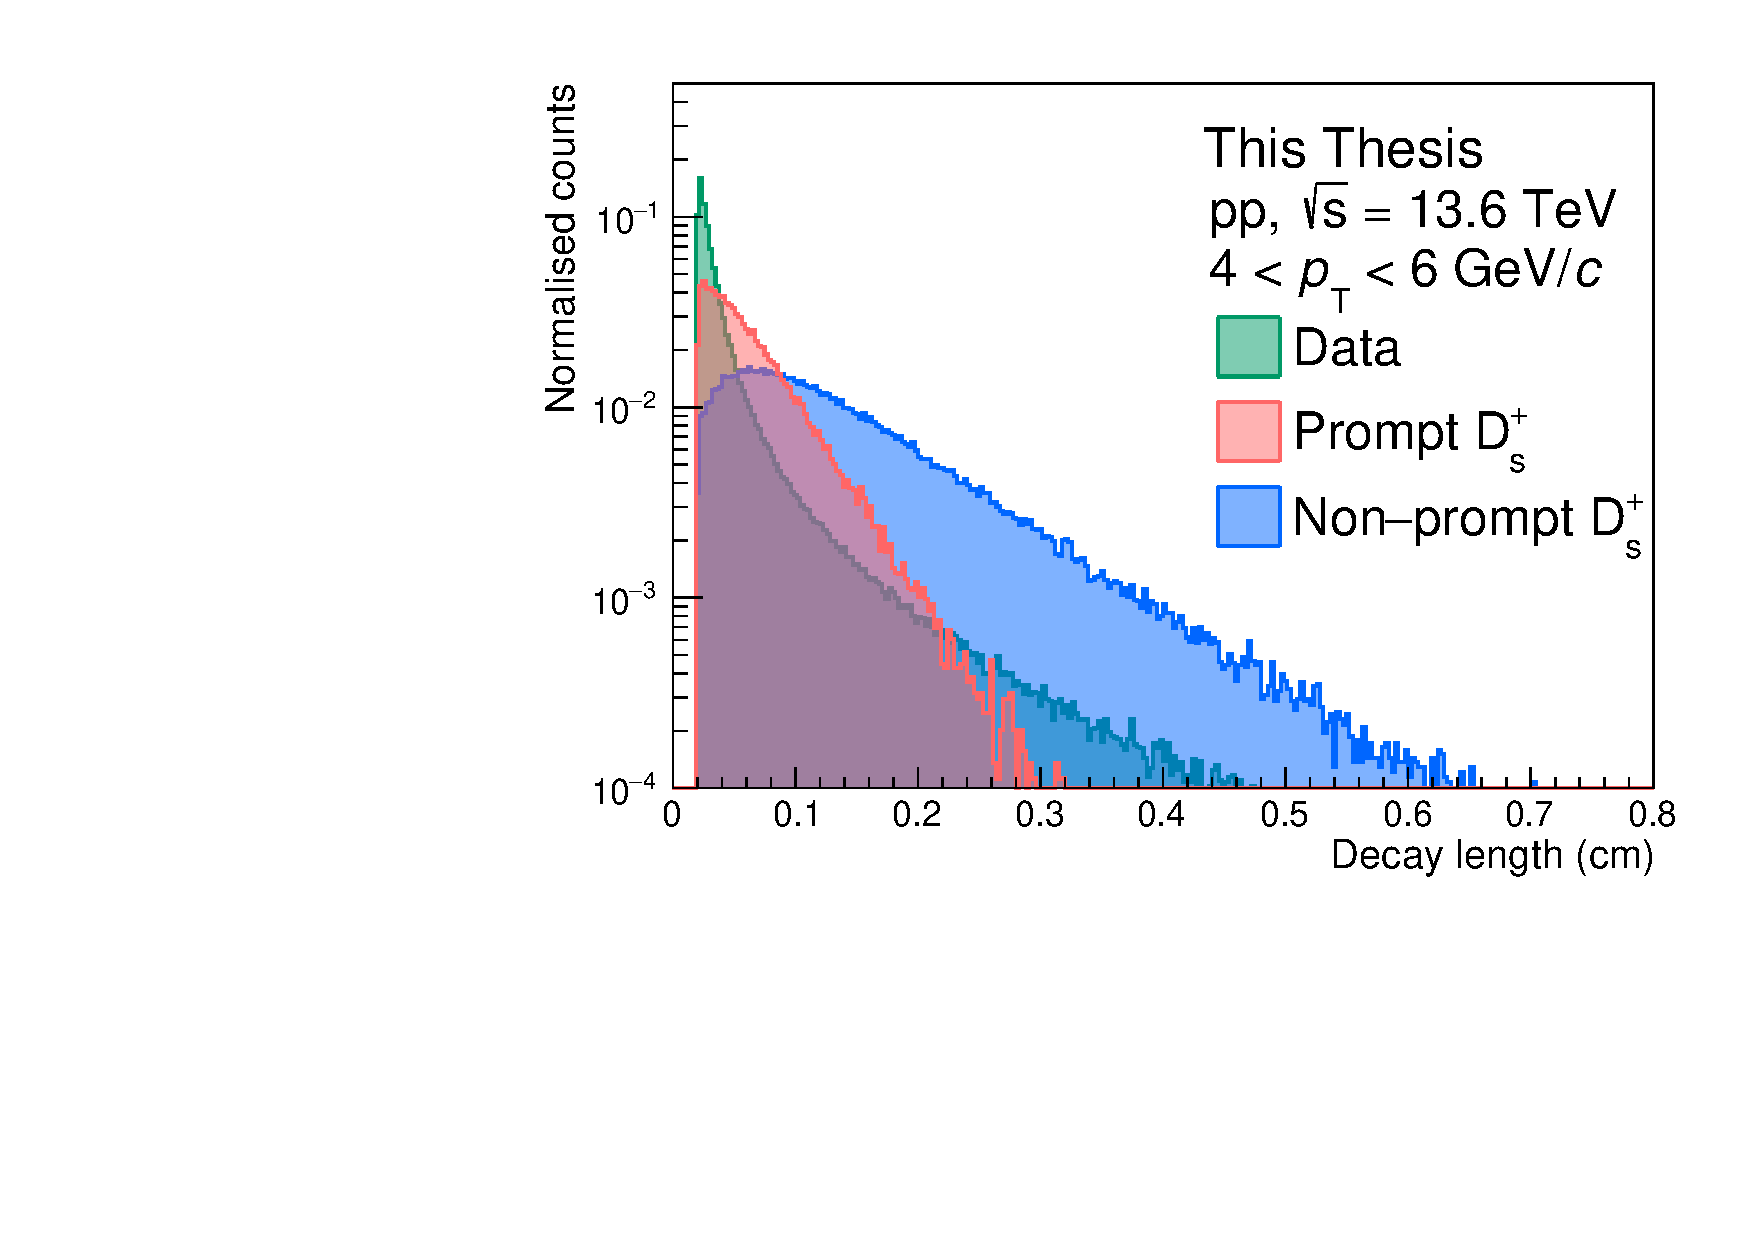
\includegraphics[width=0.48\linewidth]{Figures/Chapter 4/DecayLength.pdf}
    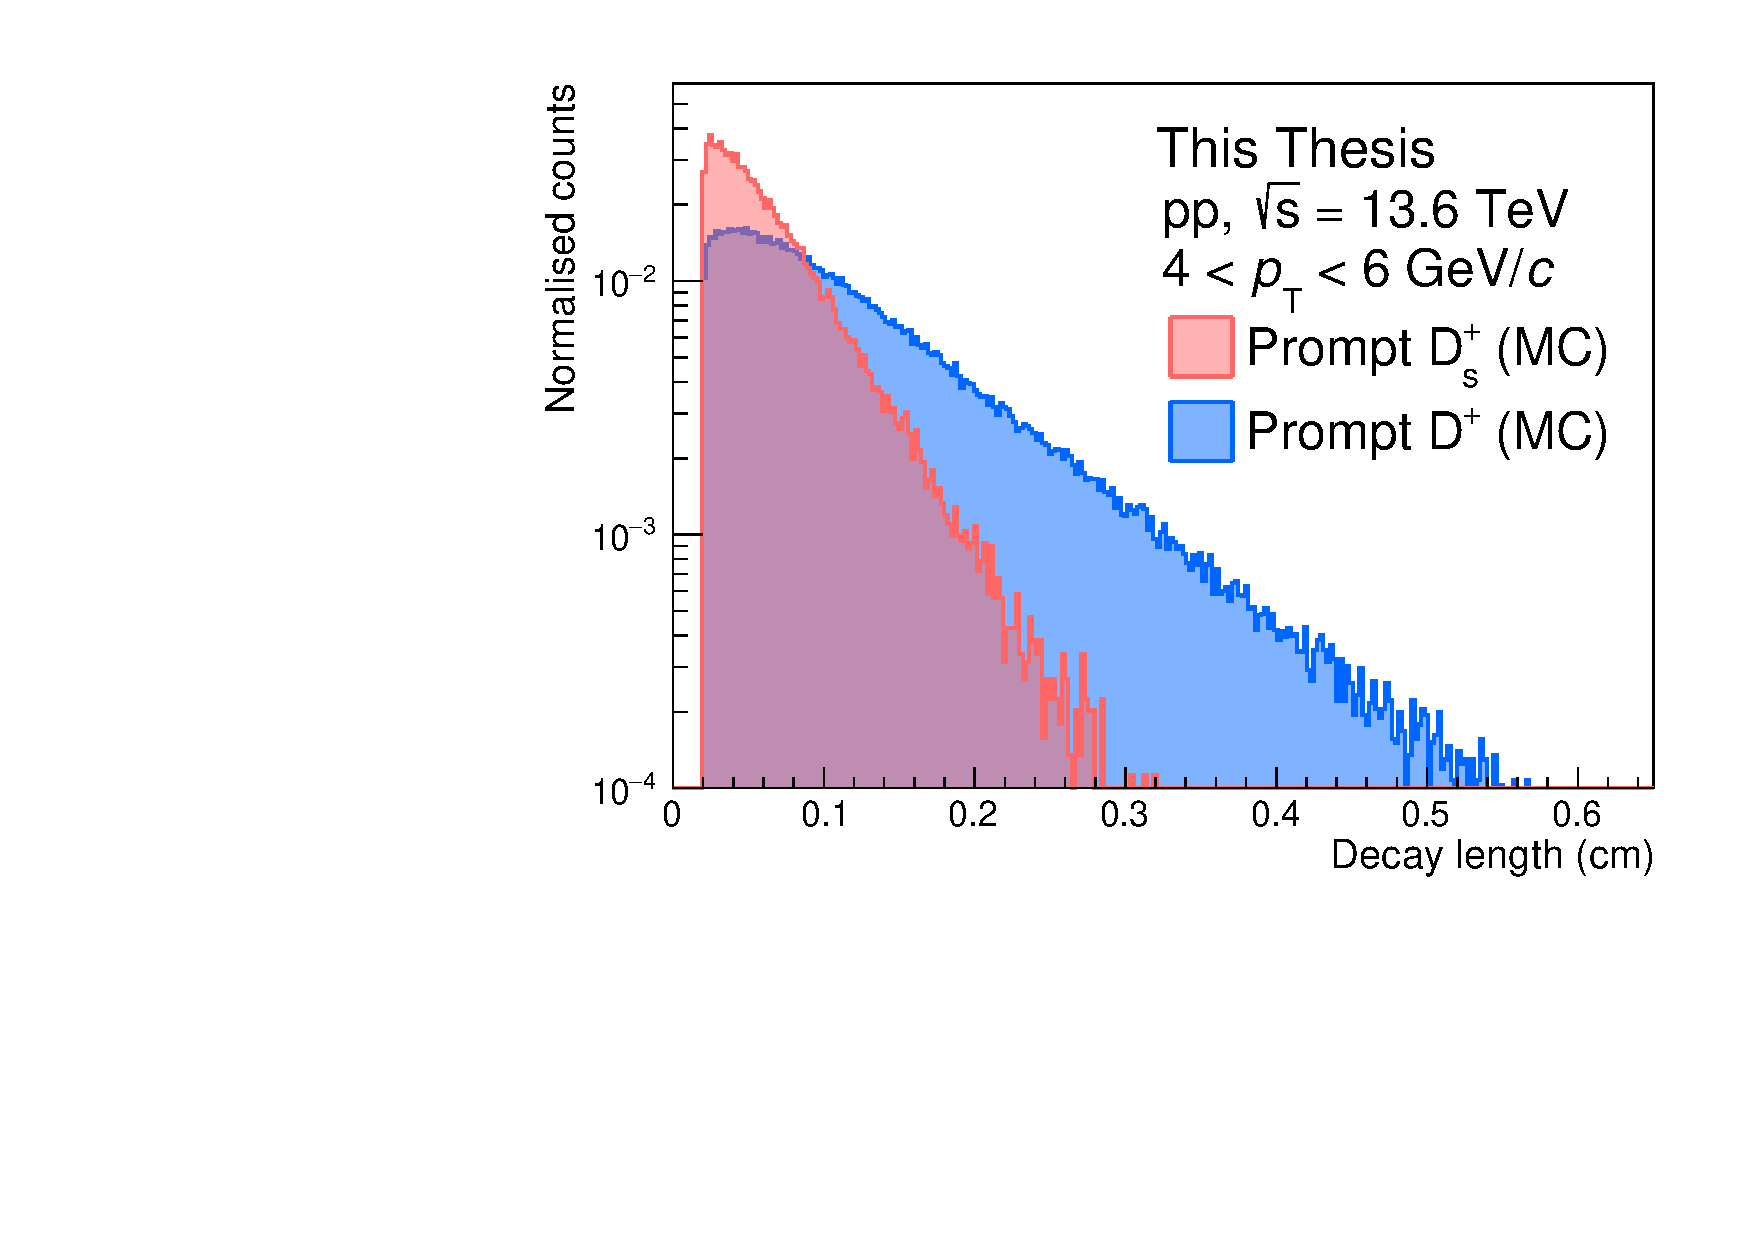
\includegraphics[width=0.48\linewidth]{Figures/Chapter 4/DecayLengthDsDPlus.pdf}
    \caption{Distributions of decay length for background (green), prompt (red), and non-prompt (blue) \ds-meson signals (left panel) and for prompt \ds- (red) and \dpl- (blue) meson signals (right panel) in pp collisions at \thirteen in the $4 < \pt < 6$~\gevc D-meson transverse momentum interval. For prompt and non-prompt \ds and \dpl mesons, the distributions are taken from Monte Carlo
    simulations, whereas for combinatorial background they are taken from the data sidebands.}
    \label{fig:DecayLength}
\end{figure}
The decay length $L$ is defined as the distance between the primary and secondary vertices. It provides an approximation of the actual decay length of \ds\ and \dpl\ mesons, as the particle's curvature resulting from the motion in the presence of a magnetic field is not considered. However, given the small mean proper decay length of $\sim 150~(310)$ µm of \ds\ (\dpl) mesons, this effect can be neglected. 

This is one of the most important variables used to distinguish between signal and combinatorial background, since the displaced topology of the signal shifts the decay length distribution towards larger values. Furthermore, since beauty-hadron decay vertices are not reconstructed, the measured decay length of non-prompt D-mesons also accounts for the decay length of their parent hadrons. As a consequence, the resulting decay length distribution for feed-down D-mesons is particularly shifted towards larger values, allowing for an easier separation of this production mechanism from the background. The distribution of the decay length also depends on the D-meson \pt, because of the Lorentz boost which contributes to an increase in the distance flown by the hadron measured in the laboratory reference frame. Moreover, since the mean proper decay length of \dpl meson is about twice as large as that of the \ds meson, the decay length distribution of the former is shifted towards larger values. Therefore, the same decay length-based selection criterion will yield different selection efficiencies for the two D-meson species.

The distributions of the decay length for cambinatorial background, prompt \ds and \dpl mesons, and for non-prompt \ds mesons are shown in Fig.~\ref{fig:DecayLength} for candidates reconstructed in the $4 < \pt < 6$~\gevc D-meson transverse momentum interval. 

In addition to the decay length, its projection on the transverse plane can also be used to select \ds or \dpl signal.\textcolor{red}{Discutere se necessario aggiungere la figura con le risoluzioni visto che è già nel capitolo precedente} %This variable is particularly useful as it exploits the better resolution of the ALICE experiment in the transverse plane with respect to the longitudinal one. 
Previous measurements of D mesons also leveraged the normalised decay length, defined as the ratio between the decay length and its uncertainty, to further improve the signal extraction. Although this variable demonstrated a good separation power, it was not used in this analysis, due to possible biases introduced by the uncertainty description in the Monte Carlo simulations.

\subsubsection{Cosine of pointing angle}
\begin{figure}[tb]
    \centering
    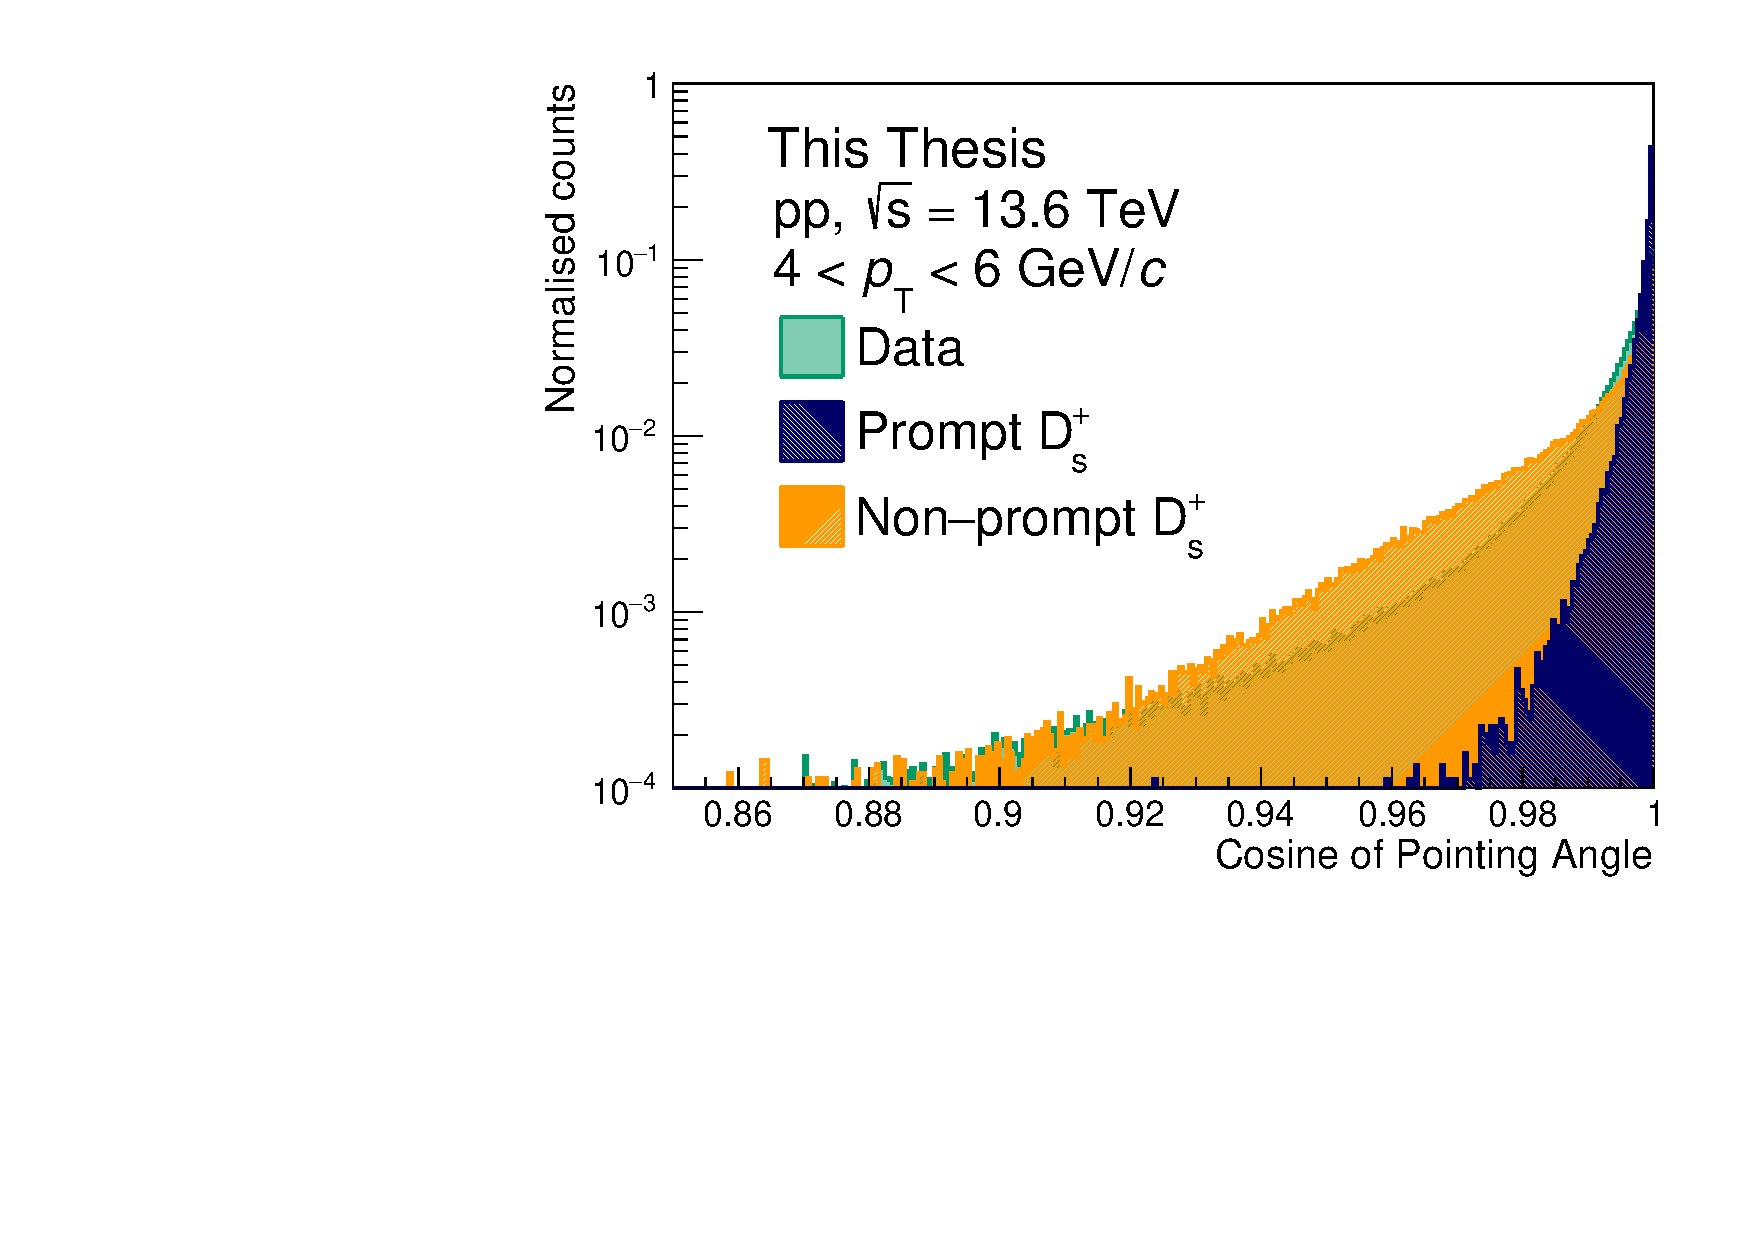
\includegraphics[width=0.48\linewidth]{Figures/Chapter 4/Cpa.pdf}
    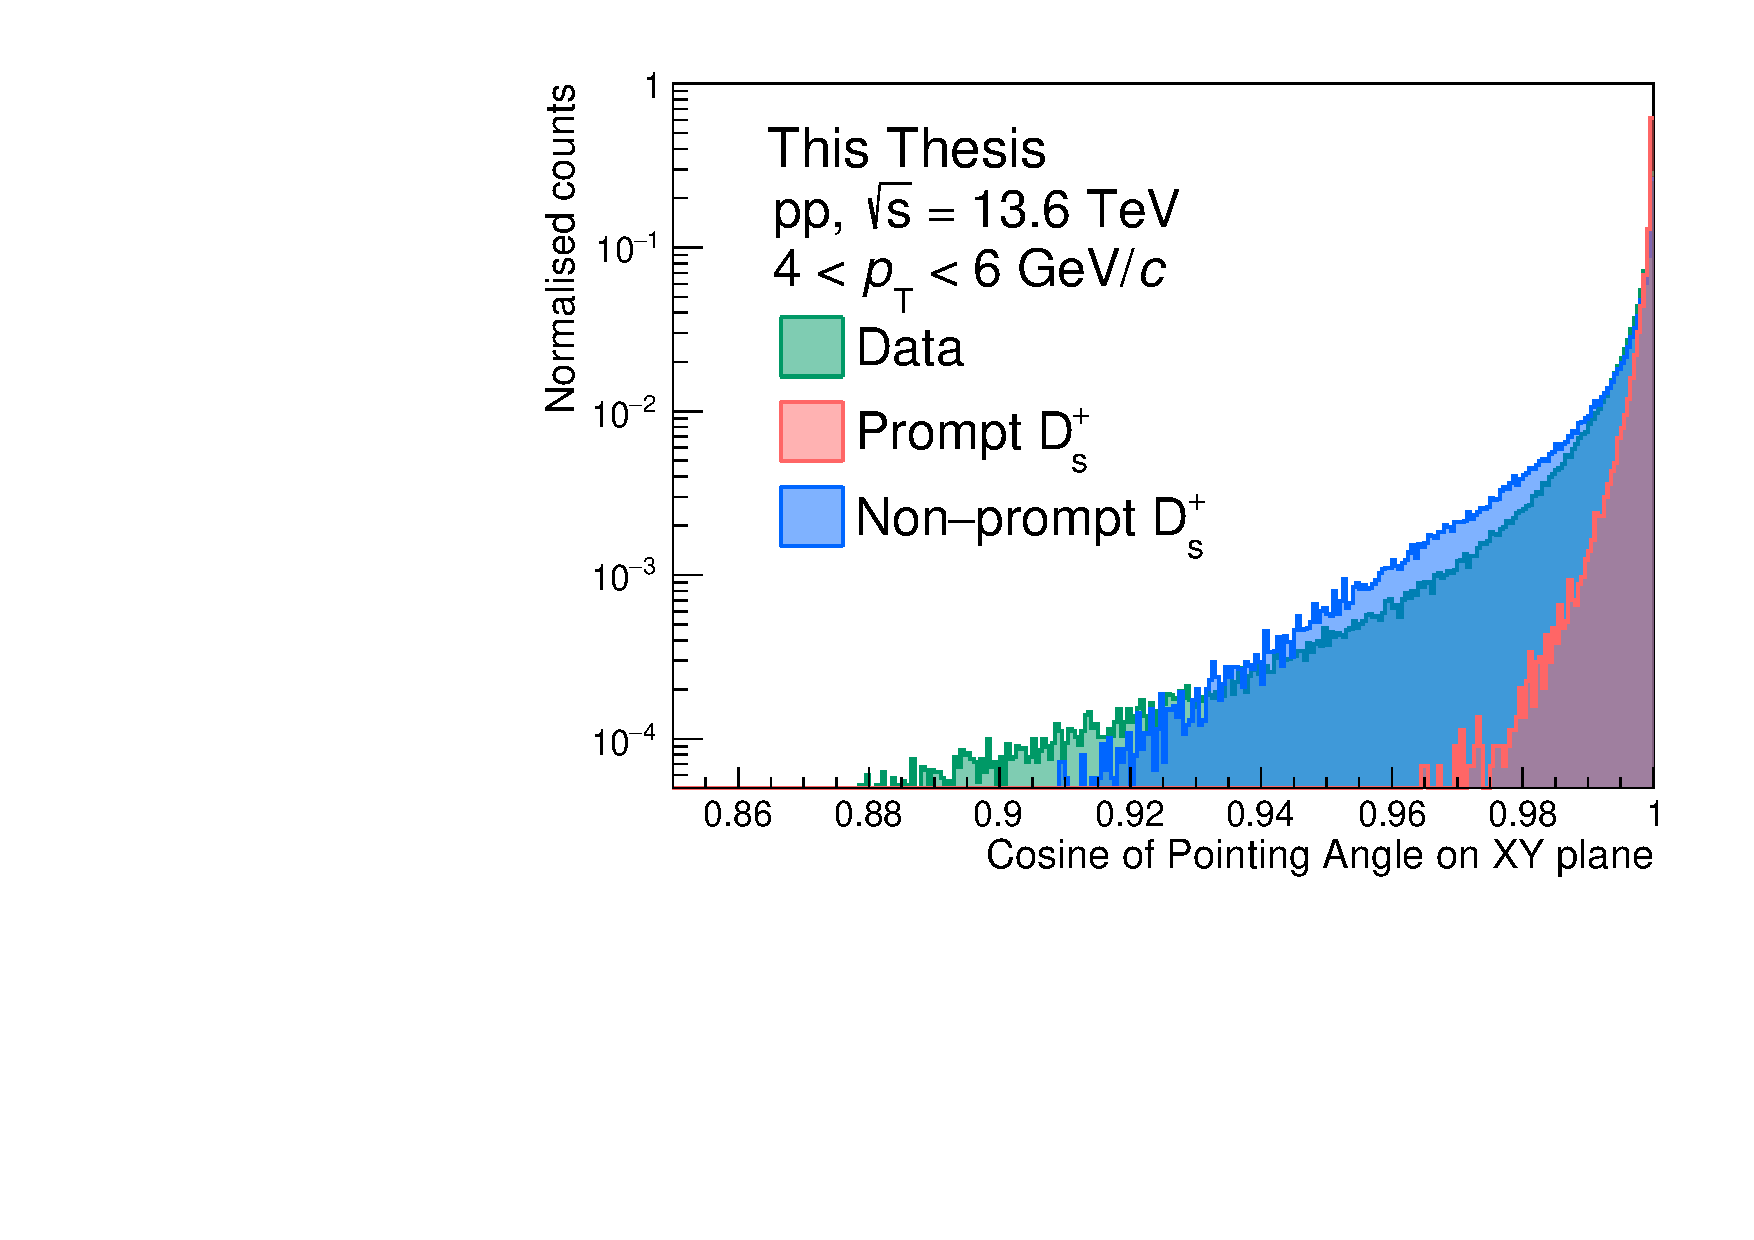
\includegraphics[width=0.48\linewidth]{Figures/Chapter 4/CpaXY.pdf}
    \caption{Distributions of the cosine of the pointing angle (left panel) and its
    projection on the transverse plane (right panel) for \ds mesons in pp collisions at \thirteen in the $4 < \pt < 6$~\gevc D-meson transverse momentum interval. The distributions are shown for prompt \ds mesons (red), non-prompt \ds mesons (blue), and combinatorial background (green). For prompt and non-prompt \ds mesons, the distributions are taken from Monte Carlo simulations, whereas for combinatorial background they are taken from the data sidebands.}
    \label{fig:PointingAngle}
\end{figure}

The pointing angle $\theta_\mathrm{p}$ is defined as the angle between the flight direction of the D meson, obtained from the line connecting the primary and secondary vertices, and the direction of the reconstructed D-meson momentum. This variable can also be defined using only the transverse components of these quantities ($\theta_\mathrm{p}^{\mathrm{xy}}$), as done for the decay length. In an ideal scenario where particles' momentum and the primary and secondary vertices are perfectly reconstructed, the cosine of the pointing angle for promptly-produced D mesons would be equal to 1, while that of feed-down D mesons would be distributed around 1, but with a tail towards lower values as the flight direction of the D meson is not equal to that of the parent beauty hadron. On the contrary, the pointing angle for combinatorial background could assume any value with the same probability. The pointing angle is therefore particularly useful to separate the signal from the combinatorial background. The distributions of the cosine of the pointing angle and its projection on the transverse plane are shown in Fig.~\ref{fig:PointingAngle} for signal and combinatorial background candidates reconstructed in the $4 < \pt < 6$~\gevc D-meson transverse momentum interval. Due to the finite resolution of the tracking detectors, the pointing angle is not perfectly reconstructed, leading to a distribution of the cosine of the pointing angle for prompt \ds that is peaked at 1, but with a tail towards lower values. The background distribution peaks at 1 as well. However, this effect is due to other applied selection criteria which select only candidates with similar features as those of the signal. 

Similarly to the decay length, also $\theta_\mathrm{p}$ evolves with the D-meson transverse momentum. Because of the Lorentz boost, the direction of the daughter particles of the D meson is more collimated with the D-meson flight direction at higher \pt. This results in a distribution of the cosine of the pointing angle that is more peaked at 1 for higher \pt values.

\subsubsection{Impact parameter in the transverse plane}
\begin{figure}[tb]
    \centering
    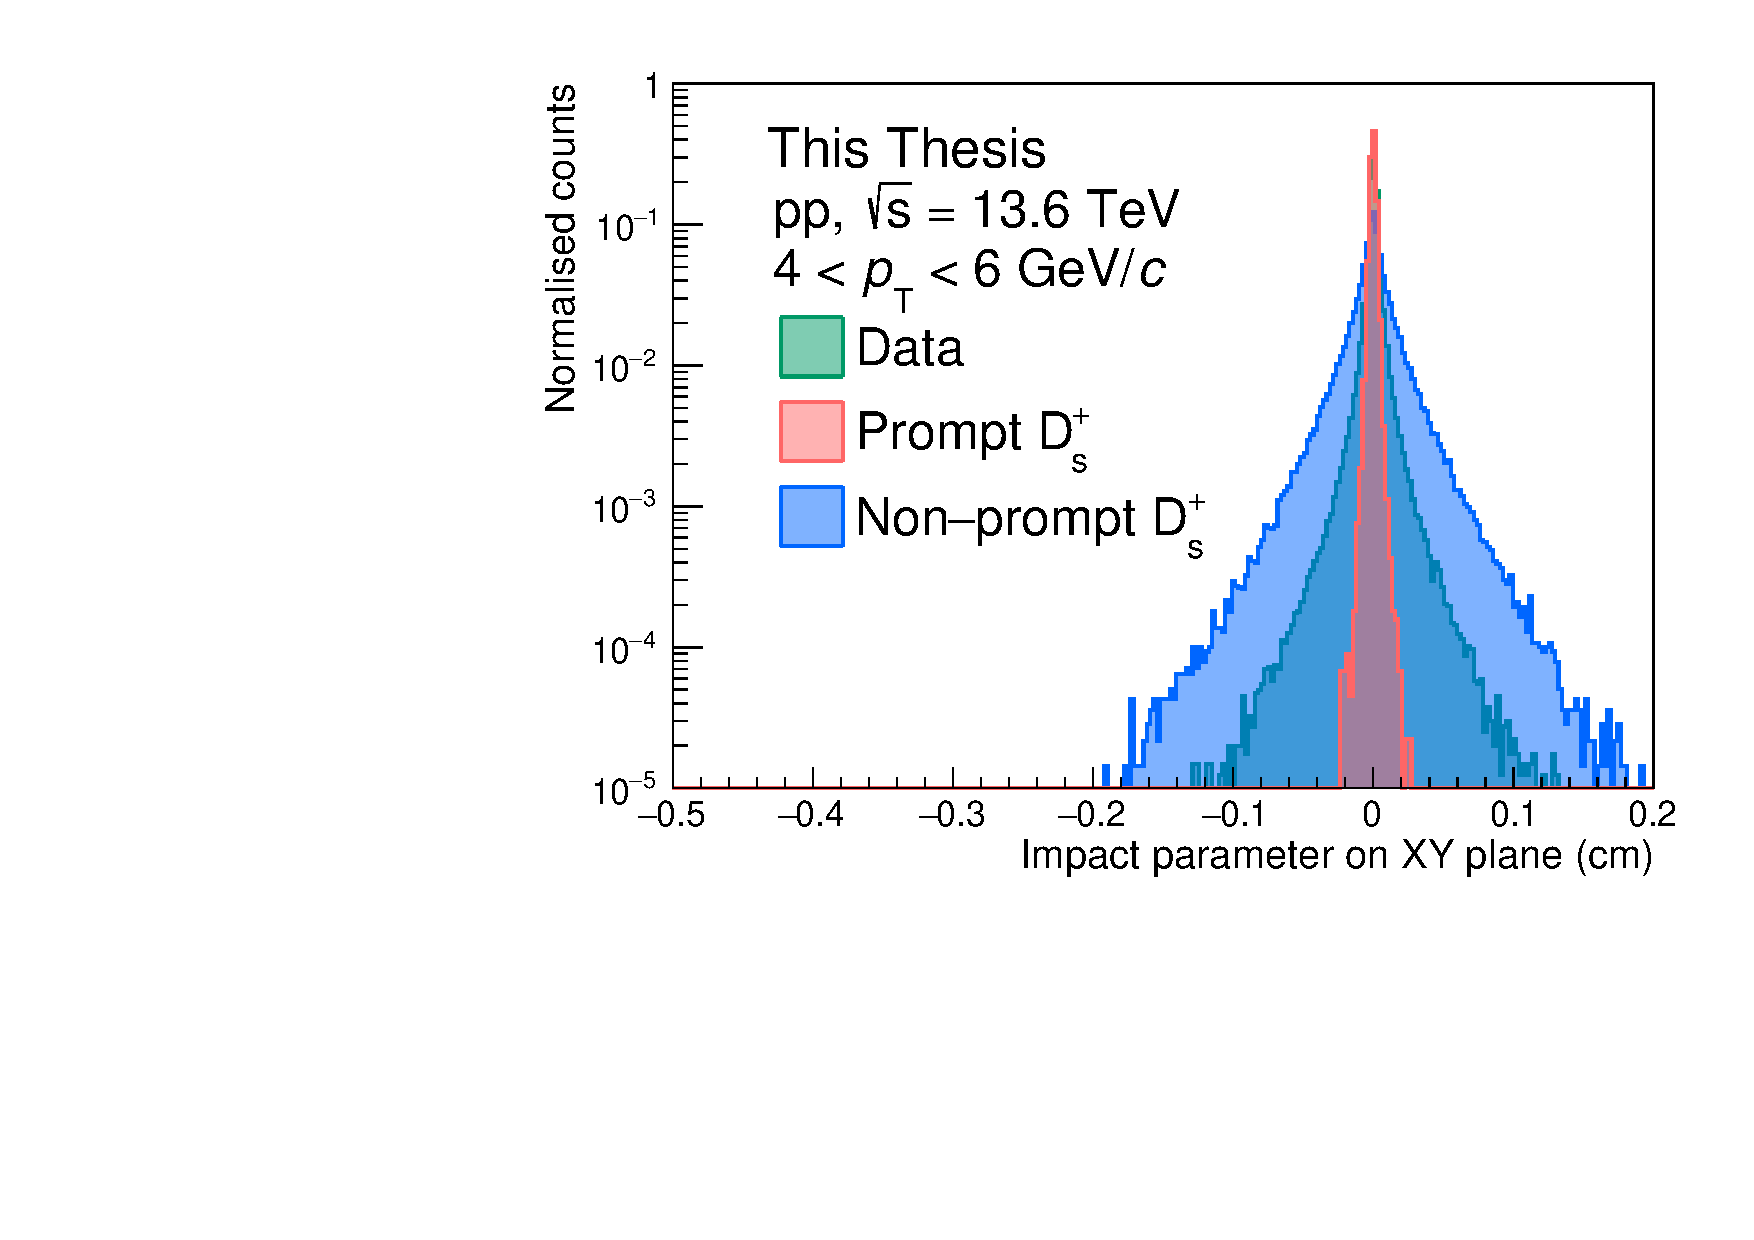
\includegraphics[width=0.48\linewidth]{Figures/Chapter 4/ImpactParameterXY.pdf}
    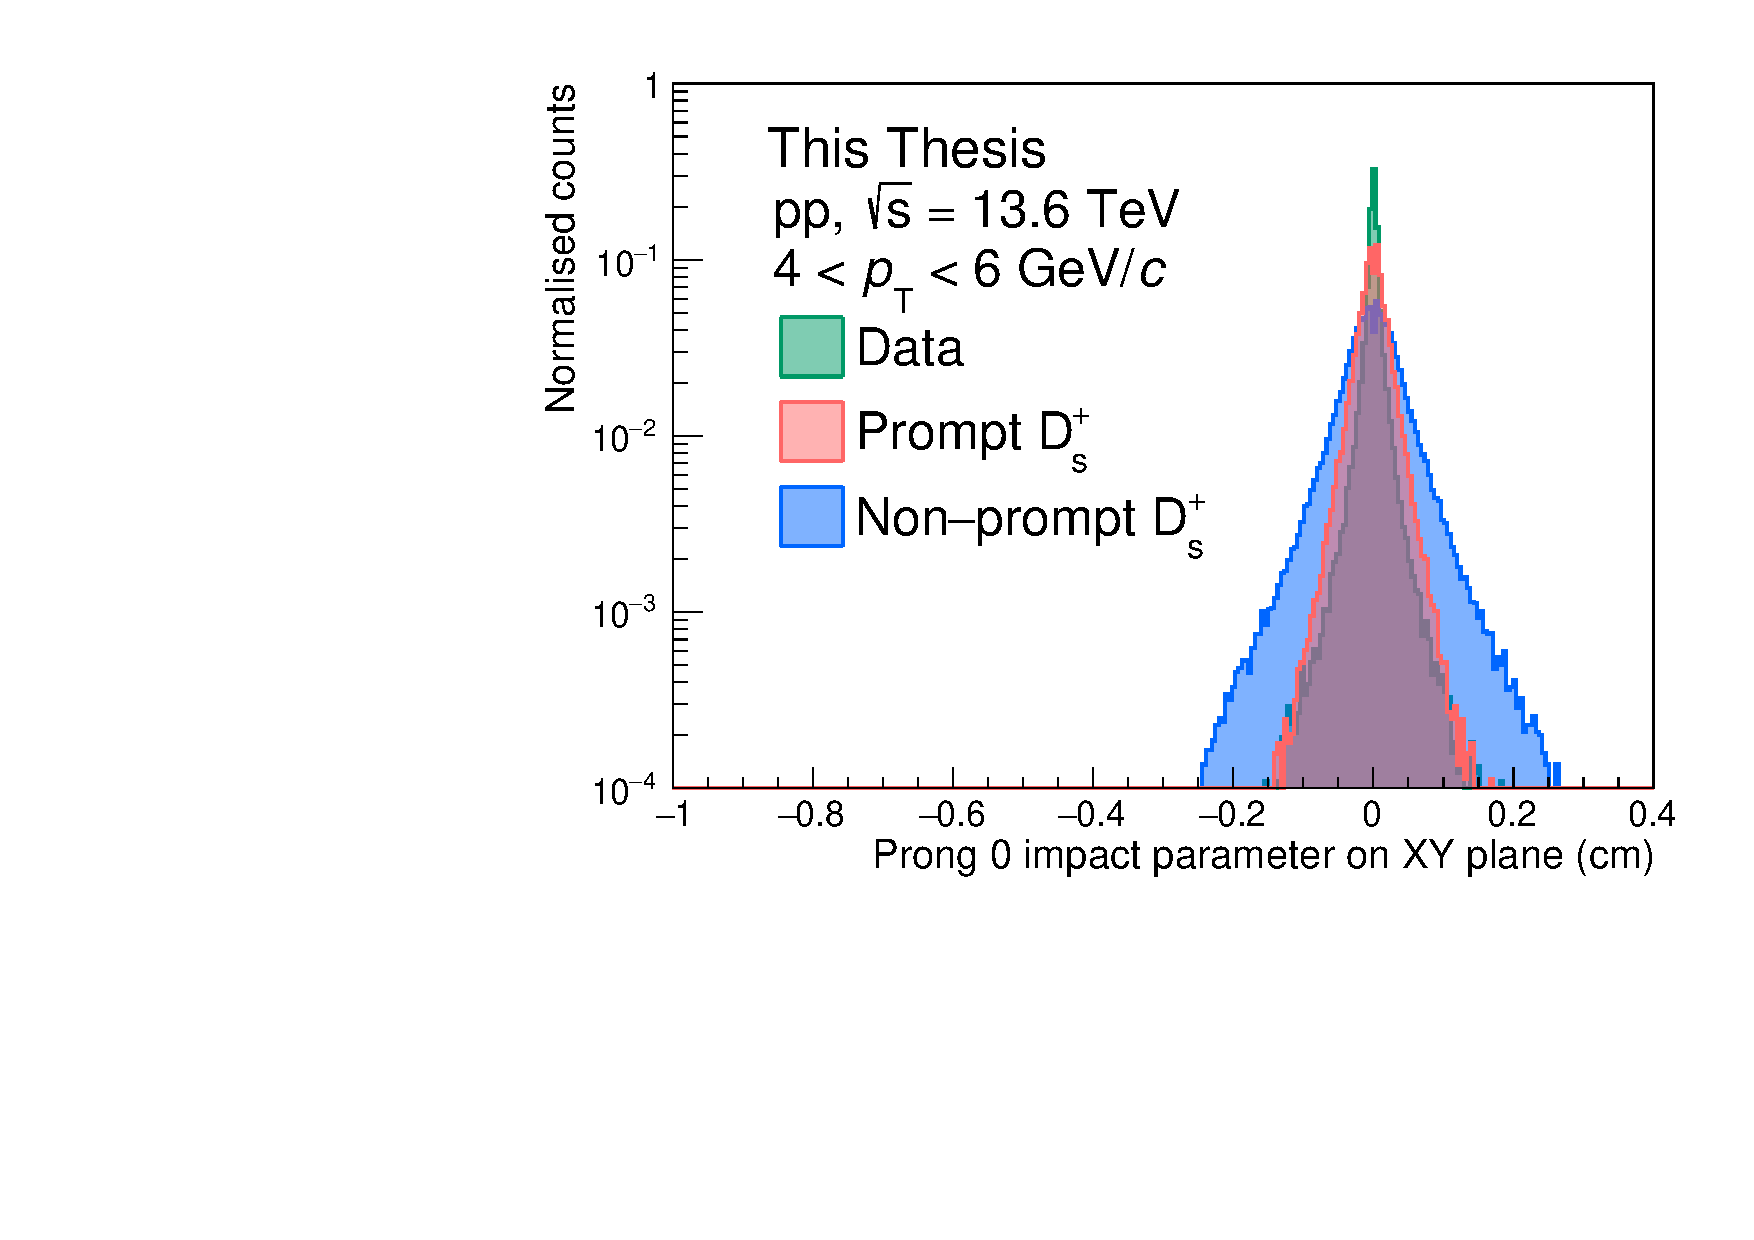
\includegraphics[width=0.48\linewidth]{Figures/Chapter 4/ImpactParameter0.pdf}
    \caption{Distributions of the projection of the impact parameter on the transverse plane for \ds mesons (left panel) and for one of the opposite-sign daughter tracks (right panel) in pp collisions at \thirteen in the $4 < \pt < 6$~\gevc D-meson transverse momentum interval. The distributions are shown for prompt \ds mesons (red), non-prompt \ds mesons (blue), and combinatorial background (green). For prompt and non-prompt \ds mesons, the distributions are taken from Monte Carlo simulations, whereas for combinatorial background they are taken from the data sidebands. }
    \label{fig:ImpactParameter}
\end{figure}
The projection of the D-meson impact parameter on the transverse plane $d_0^{xy}$ is defined as the distance of closest approach between the reconstructed flight line of the D-meson and the primary vertex, projected in the $xy$ plane. It is expected to be very close to zero for promptly-produced D mesons, with any deviation due to the detector resolution. Thanks to the better momentum and vertexing resolution, its distribution becomes narrower at high \pt. It is a powerful variable not only to separate the signal from the combinatorial background, but also to discriminate between prompt and feed-down D mesons, as the latter have a much broader impact parameter distribution, as shown in the left panel of Fig~\ref{fig:ImpactParameter}. In addition, also the projection of the daughter tracks' impact parameter to the primary vertex projected on the transverse plane is used to select the signal. Since combinatorial-background candidates are mostly composed of tracks originating from the primary vertex, a narrow distribution around 0 is expected for the prongs' impact parameters of such candidates. On the contrary, the displaced decay vertex of the signal candidates leads to a broader distribution of the impact parameter for prompt D-meson candidates, and to an even broader one for the non-prompt contribution to the signal, as shown in the right panel of Fig.~\ref{fig:ImpactParameter}.

\subsection{Kinematic selections}
In addition to the selections based on the decay topology, kinematic selections are also applied to increase the signal-over-background ratio and the statistical significance of the measurement.
\begin{figure}[tb]
    \centering
    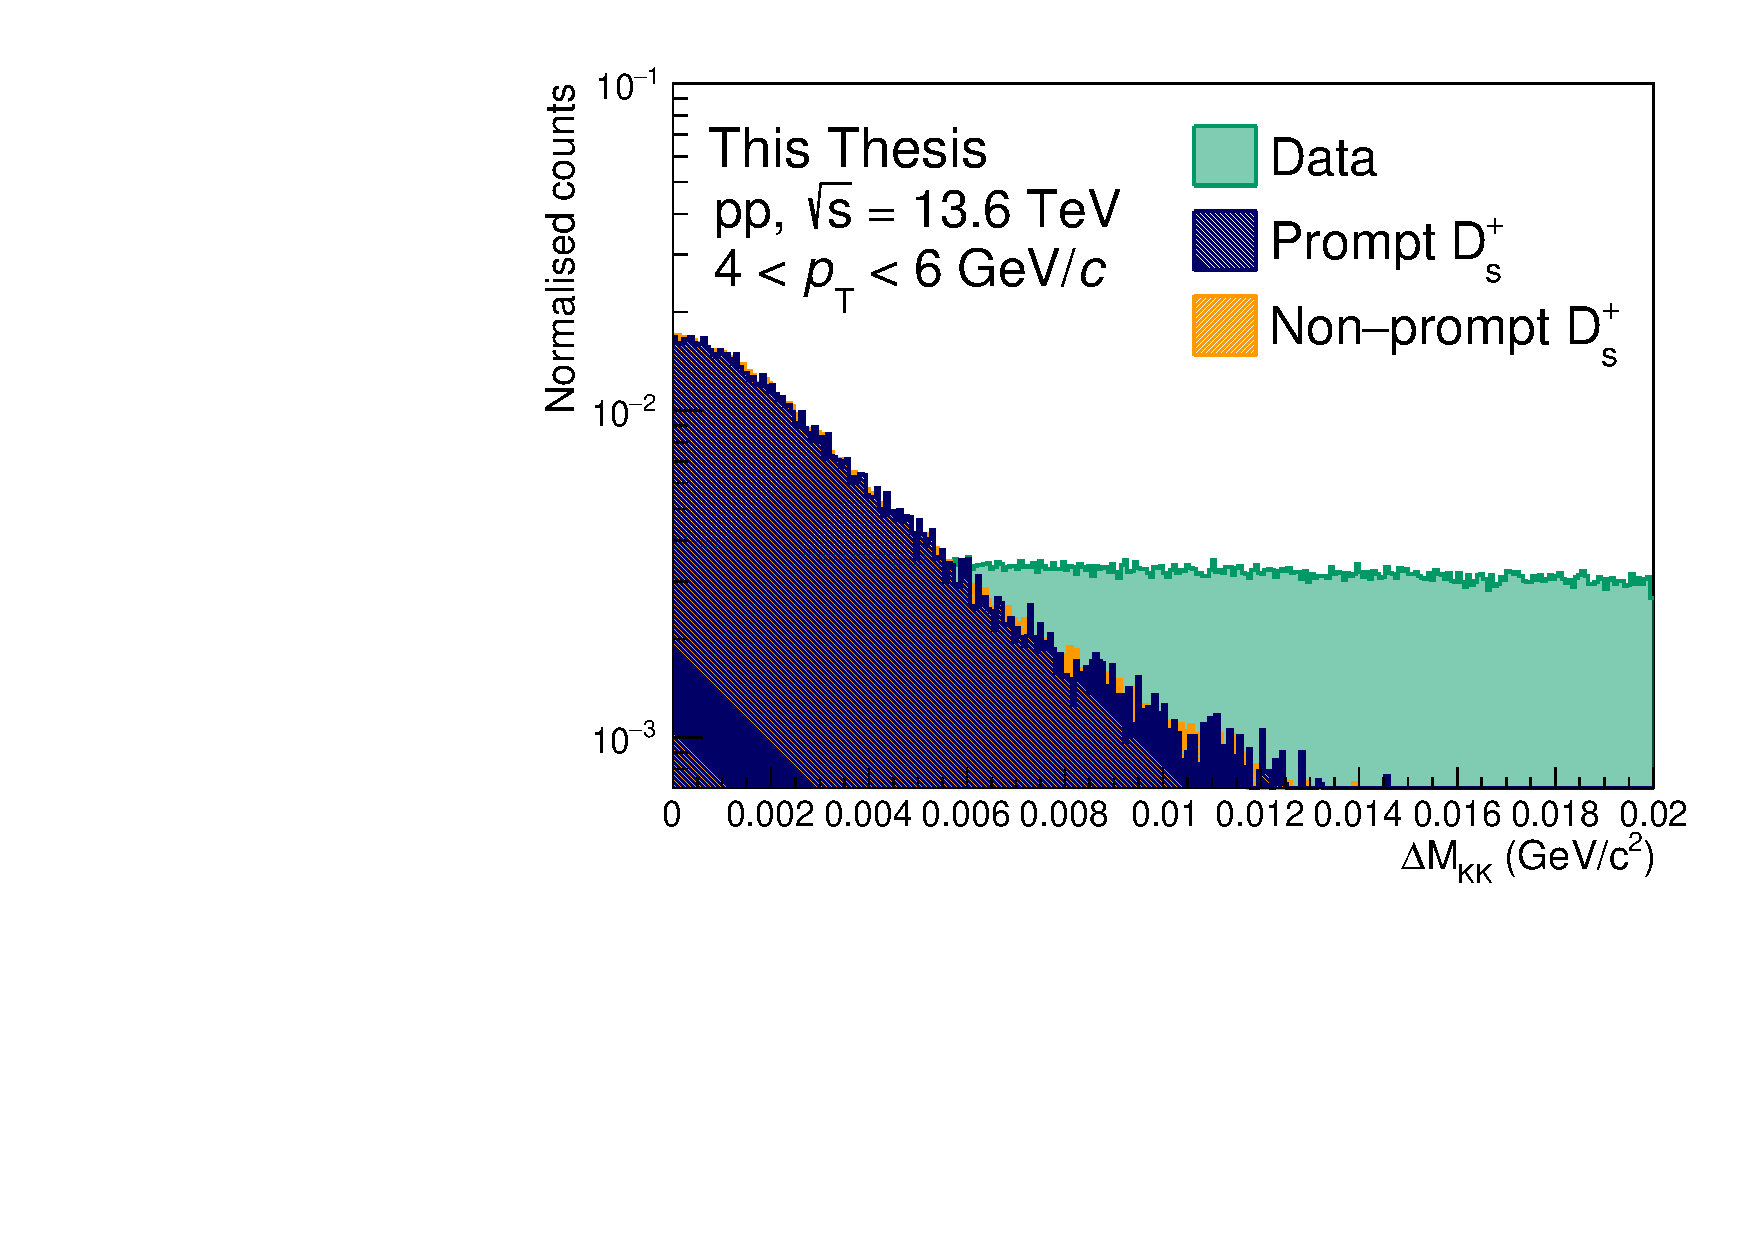
\includegraphics[width=0.48\linewidth]{Figures/Chapter 4/DeltaMassKK.pdf}
    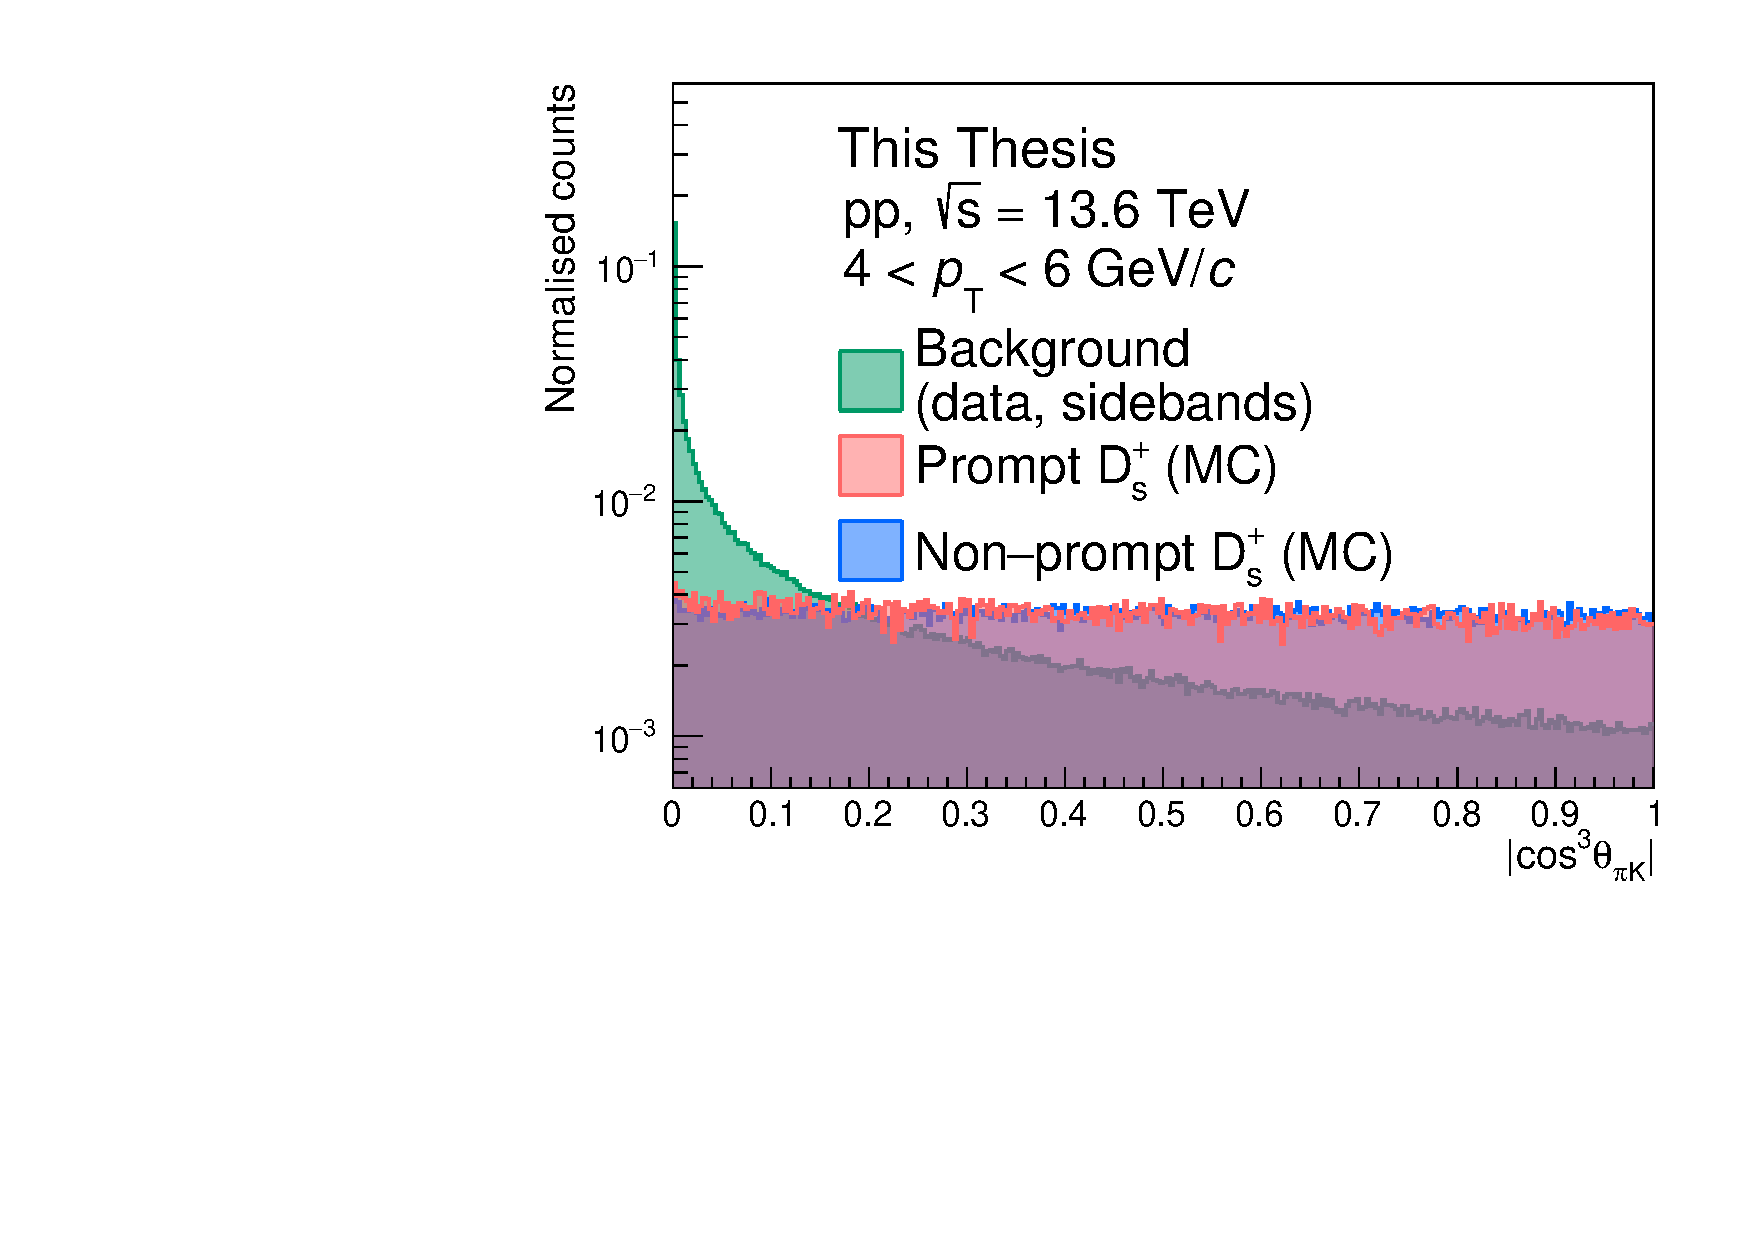
\includegraphics[width=0.48\linewidth]{Figures/Chapter 4/AbsCos3PiK.pdf}
    \caption{Distributions of the difference between the reconstructed $\mathrm{K^+K^-}$ invariant mass and the PDG mass of the $\phi$ meson (left panel) and the cosine cubed of the K-$\pi$ angle in the KK rest frame (right panel) for \ds mesons in pp collisions at \thirteen in the $4 < \pt < 6$~\gevc D-meson transverse momentum interval. The distributions are shown for prompt \ds mesons (red), non-prompt \ds mesons (blue), and combinatorial background (green). For prompt and non-prompt \ds mesons, the distributions are taken from Monte Carlo simulations, whereas for combinatorial background they are taken from the data sidebands.}
    \label{fig:DeltaMassPhi}
\end{figure}

\subsubsection{Difference between reconstructed and PDG mass of the \boldmath$\phi$ meson}
\begin{sloppypar}
This selection exploits the production of an intermediate resonant $\phi(1020)$-meson state in the considered decay channel of the D mesons, which is characterised by an invariant mass of \mbox{$M_\phi = (1019.461\pm0.016)$}~\mevcc and a narrow resonance peak of $\Gamma_\phi = 4.249\pm0.013$~\mevcc~\cite{pdg}. Therefore, the difference between the reconstructed invariant mass of the $\mathrm{K^+K^-}$ pair and the PDG mass of the $\phi$ meson $\lvert\Delta M(\mathrm{KK})\rvert$ is expected to be close to zero for signal candidates, while the distribution for combinatorial background is expected to be uniformly distributed.
\end{sloppypar}
Moreover, two possible $\mathrm{K^+K^-}$ pairs can be built for each triplet of tracks, depending on the mass hypothesis assigned to the like-sign tracks (e.g., for a \ds decay, both the $\mathrm{K^+K^-\pi^+}$ and $\mathrm{\pi^+K^-K^+}$ mass hypotheses can be considered). Both hypotheses are considered in the reconstruction, and the selection on $\lvert\Delta M(\mathrm{KK})\rvert$  results extremely helpful not only in rejecting the combinatorial background, but also the reflections, i.e., D mesons with wrongly-assigned mass hypothesis to the decay tracks.


The distribution of this variable is shown in the left panel of Fig.~\ref{fig:DeltaMassPhi} for signal and combinatorial background candidates reconstructed in the $4 < \pt < 6$~\gevc D-meson transverse momentum interval.

\subsubsection{Cosine cubed of the K-\boldmath$\pi$ angle in the KK rest frame}
The decay of a (pseudoscalar) D-meson to a (vector) $\phi$-meson and a (pseudoscalar) $\pi^+$ final state results in an alignment of the spin of the $\phi$ meson with respect to the direction of motion of the $\phi$ relative to the D-meson~\cite{ZEUS:2000rhm}. As a consequence, the distribution of $\mathrm{cos}\left(\theta'(\mathrm K)\right)$, where $\theta'(\mathrm K)$ is the angle between one of the kaons and the pion in the $\mathrm{K^+K^-}$
rest frame, follows a $\mathrm{cos}^2\left(\theta'(\mathrm K)\right)$ shape, which in turn implies a flat distribution for the $\mathrm{cos}^3\left(\theta'(\mathrm K)\right)$ variable, in case of signal. In contrast, the combinatorial background has a flat distribution for $\cos\left(\theta'(\mathrm K)\right)$, and its $\cos^3\left(\theta'(\mathrm K)\right)$ distribution peaks at zero. This variable is particularly useful to separate the signal from the combinatorial background, as shown in the right panel of Fig.~\ref{fig:DeltaMassPhi}.

\subsection{Particle identification selections}\label{sec:PIDselections}
One of the distinctive features of the ALICE detector is the excellent PID capabilities in a wide range of momentum, achieved by combining the information from different detectors. 
The TPC is the main PID detector in the ALICE experiment, as it provides a simultaneous measure of the specific energy loss via the charge produced in the drift volume and deposited in its 159 pad rows, the charge, and the momentum of each particle traversing the detector gas. A truncated mean of the \dedx samples is calculated discarding the 40\% highest-charge clusters, which ensures the removal of the Landau tail of the \dedx distribution caused by $\delta$-rays, which are produced from the ionisation of the gas by the electrons produced in the primary ionisation. The particle identification is based on the comparison of the measured \dedx with the expectation for a specific particle species with a certain momentum $p$. The expected \dedx is described by the Bethe-Bloch formula, and is typically parametrised with a function originally proposed by the ALEPH collaboration~\cite{Blum:2008nqe}:
\begin{equation*}
    f(\beta\gamma) = \frac{P_1}{\beta^{P_4}}\left[P_2 - \beta^{P_4} - \log\left(P_3 + \frac{1}{(\beta\gamma)^{P_5}}\right)\right]\quad .
\end{equation*}
In this parametrisation, $\beta$ and $\gamma$ are the particle velocity and Lorentz factor, respectively, and $P_{1-5}$ are the parameters of the fit function. The \dedx distribution in the TPC is shown in the right panel of Fig.~\ref{fig:ITSTPCPID} for pp collisions at \thirteen. The curves obtained with a fit using the ALEPH parametrisation of the Bethe-Bloch formula for electrons, muons, pions, kaons, protons, deuterium, and tritium are also shown. While in the non-relativistic low momentum region ($p \leq 1$~\gevc) p, K, and $\mathrm{\pi}$ can be separated on a track-by-track basis, at higher momenta, in the relativistic rise region, particles can still be identified on a statistical basis via multi-Gaussian fits~\cite{ALICE:2014sbx}. This is possible because the truncated-mean method produces a \dedx peak with a gaussian shape down to three orders of magnitude for long tracks (at least 130 clusters)~\cite{ALICE:2014sbx}.
\begin{figure}[htb]
    \centering
    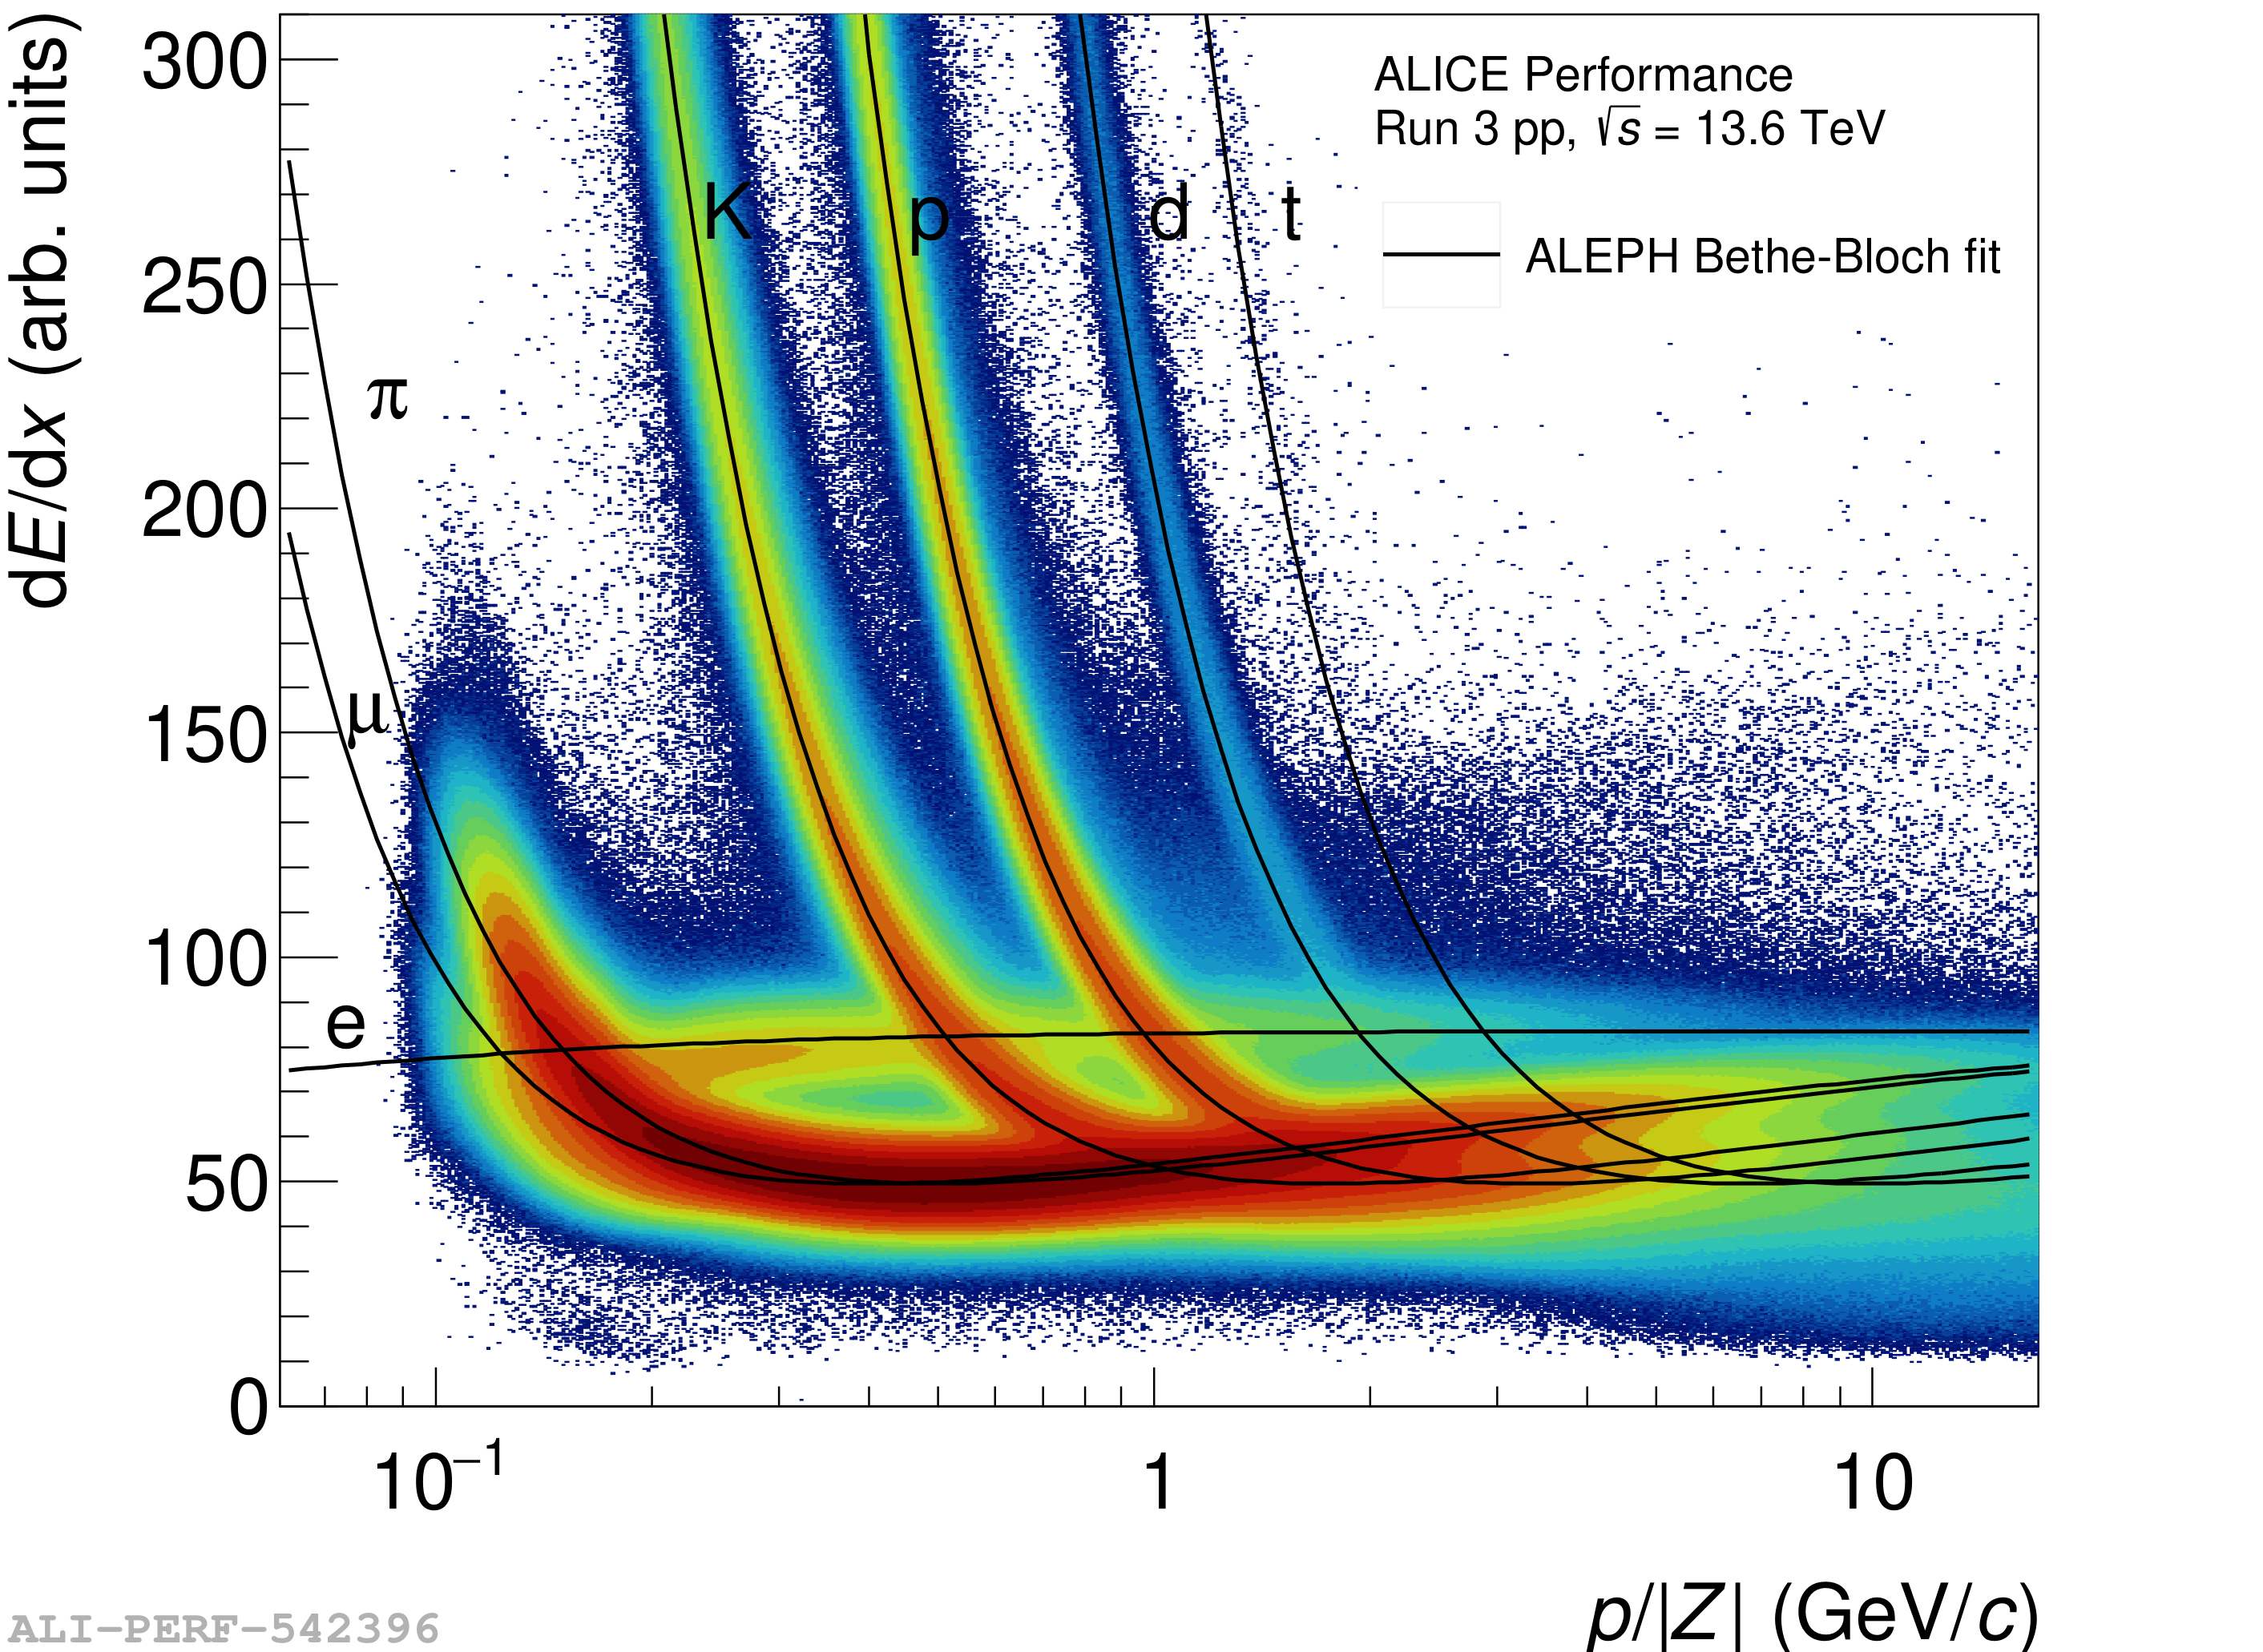
\includegraphics[width=0.7\linewidth]{Figures/Chapter 4/tpcdedx_1.png}
    \caption{Specific energy loss distribution \dedx in the TPC for pp collisions at \thirteen. The curves obtained with a fit using the ALEPH parametrisation of the Bethe-Bloch formula for electrons, muons, pions, kaons, protons, deuterium, and tritium are also shown. Figures taken from the ALICE figure repository~\cite{ALICE_figures}.}
    \label{fig:ITSTPCPID}
\end{figure}

The TOF detector is dedicated to PID in the intermediate momentum range, up to 2.5~\gevc for pions and kaons, and up to 4~\gevc for protons. In this higher-\pt region, the TPC is not able to provide a sufficient separation between the different particle species. The TOF detector is based on the measurement of the time of flight of charged particles between the interaction point and the detector. The start time is provided by the FT0 forward-rapidity detectors, and a total time resolution of about 80~ps is achieved, allowing for a separation of the different particle species based on the time of flight. The TOF PID performance is shown in Fig.~\ref{fig:TOFPID} for pp collisions at \thirteen. The large background is due to tracks that are incorrectly matched to TOF hits in high-multiplicity \pbpb collisions.

\begin{figure}[htb]
    \centering
    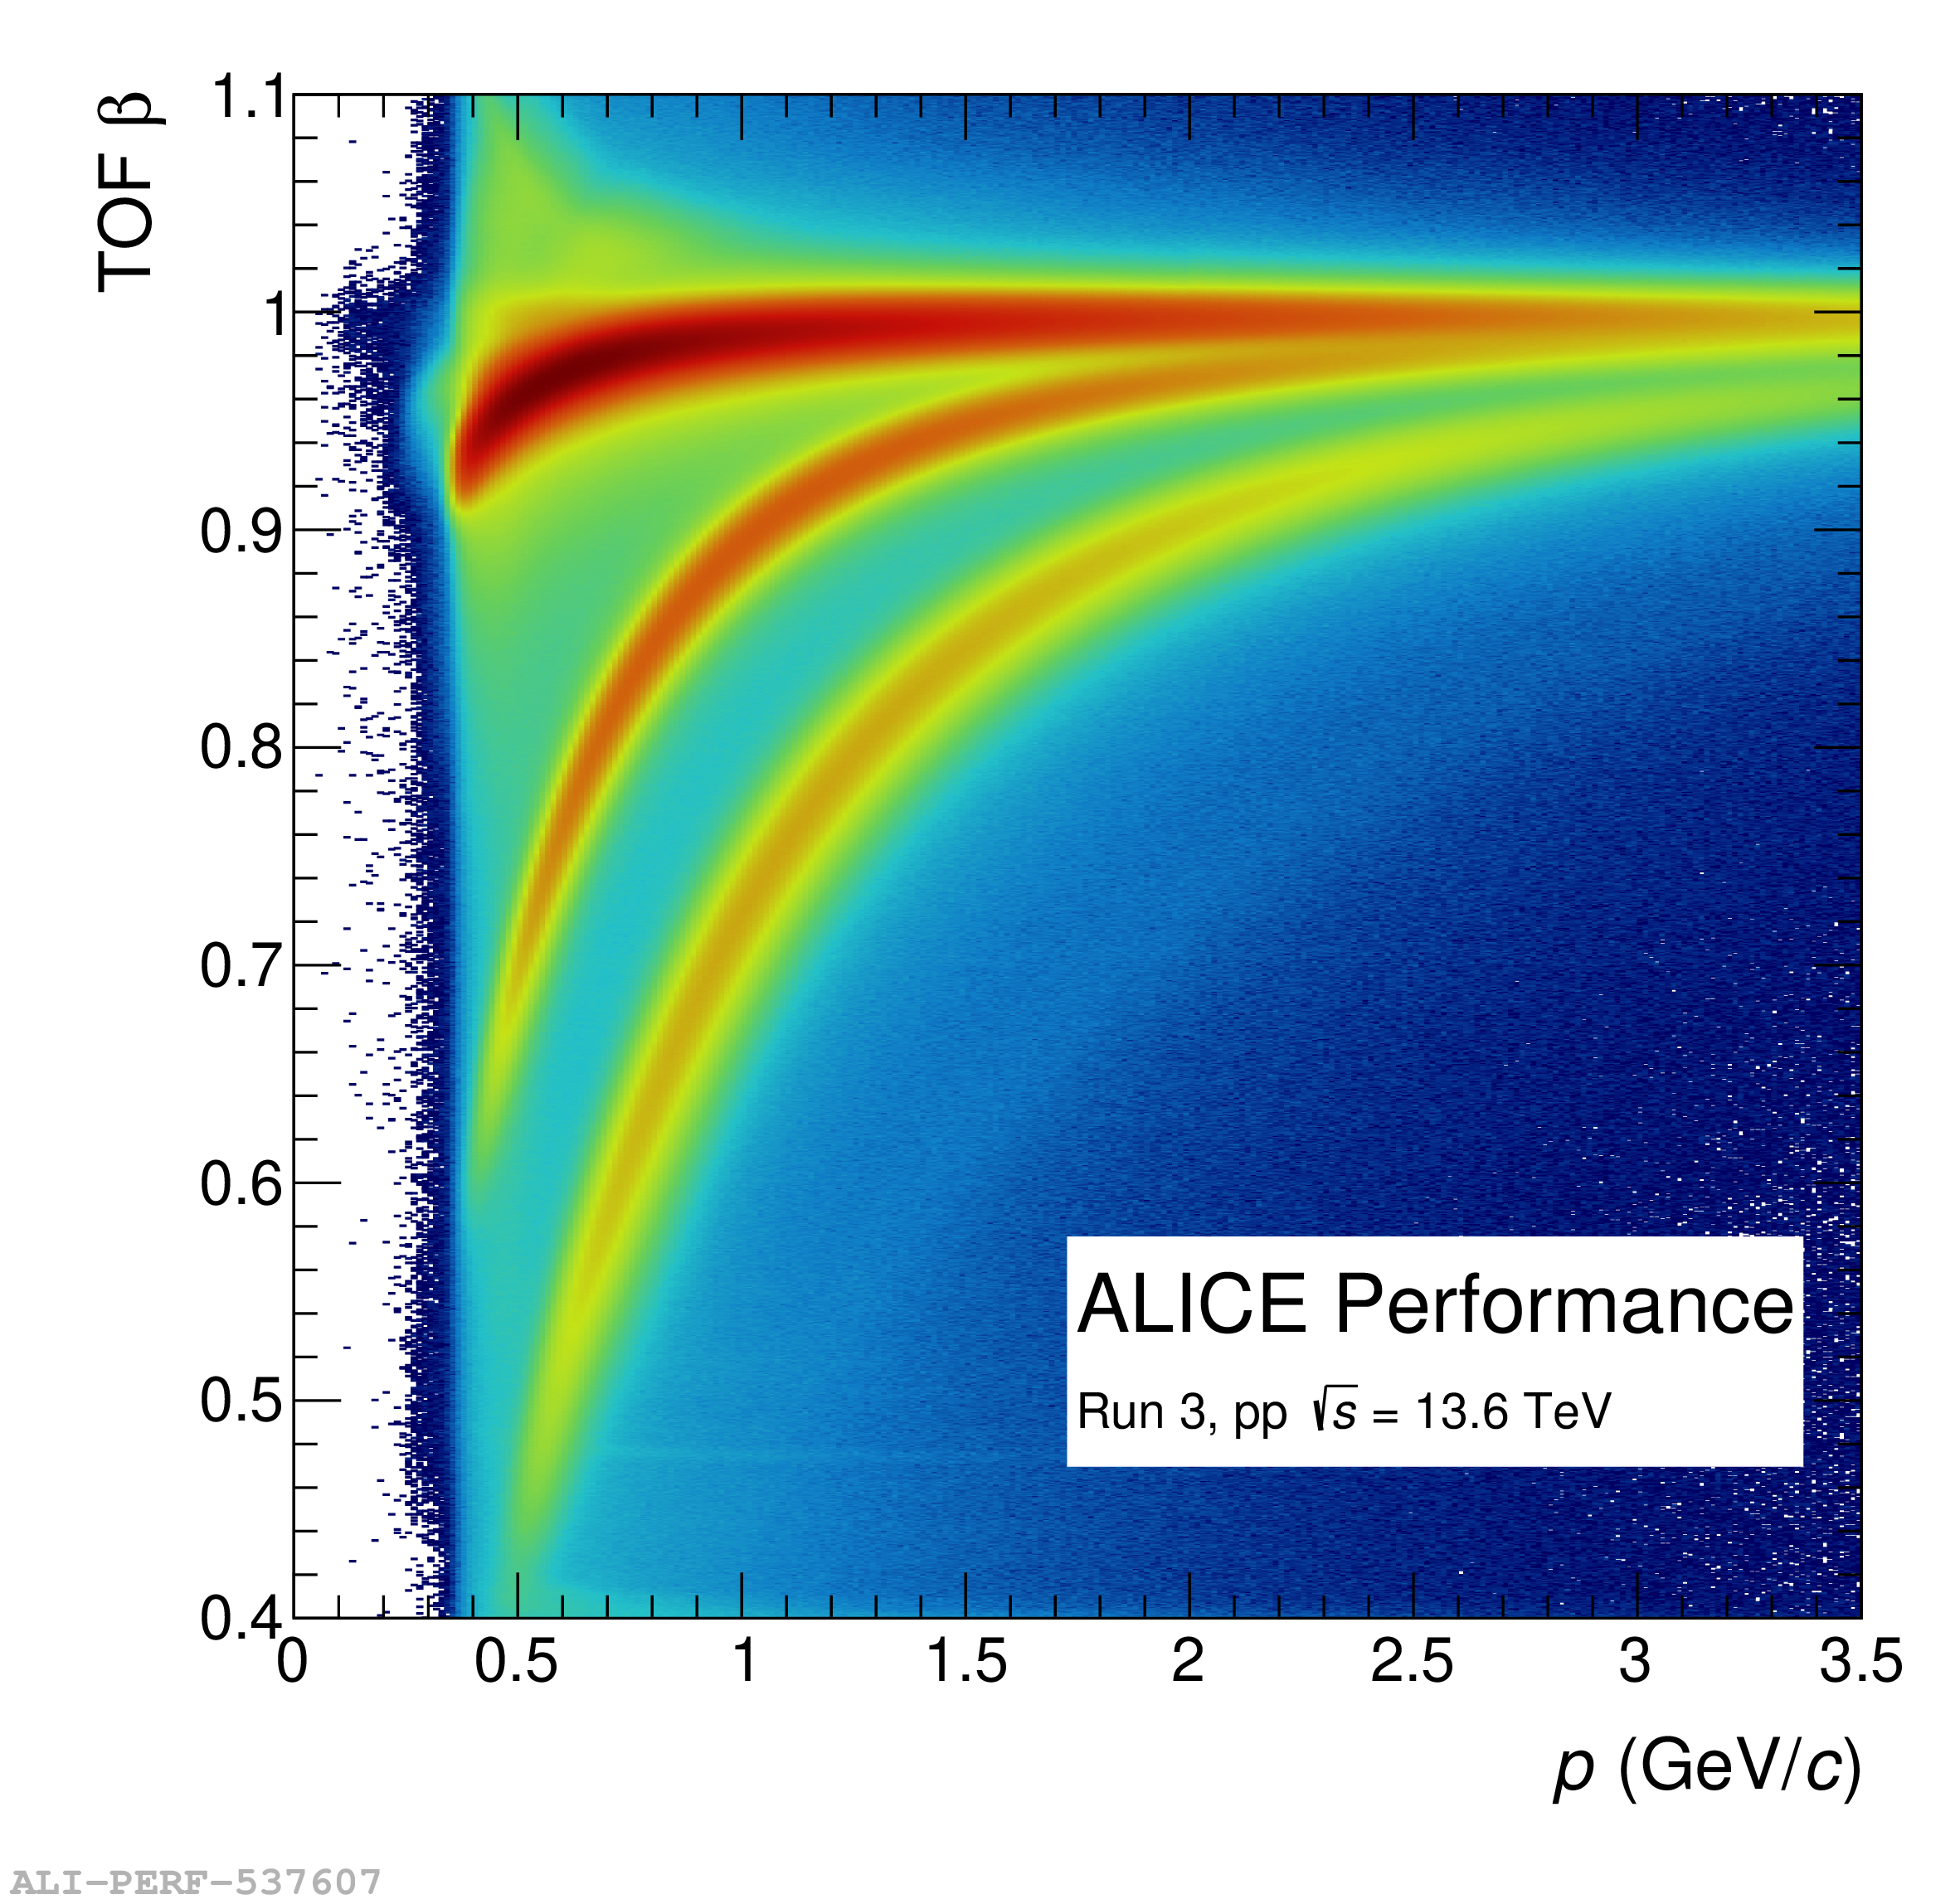
\includegraphics[width=0.7\linewidth]{Figures/Chapter 4/toflhc22q_pass3_0.png}
    \caption{$\beta$ parameter measured with the TOF detector as a function of the momentum $p$ measured by the TPC detector in pp collisions at \thirteen. Figure taken from the ALICE figure repository~\cite{ALICE_figures}.}
    \label{fig:TOFPID}
\end{figure}

%Other detectors, such as the High Momentum Particle Identification Detector (HMPID) or the Transition Radiation Detector (TRD), complement the PID capabilities of the ALICE experiment. The HMPID is dedicated to the identification of particles with momenta above 2~\gevc, and is based on the detection of Cherenkov radiation emitted by charged particles traversing a radiator. The TRD is used for the identification of electrons and positrons, and is based on the detection of transition radiation emitted by charged particles traversing a radiator with a change in the dielectric constant. The TRD is particularly useful for the identification of electrons and positrons in the high-multiplicity environment of heavy-ion collisions, where the TPC and TOF detectors are not able to provide a sufficient separation between electrons and pions. 

The PID information on the decay tracks can be exploited in the D-meson selection to improve the background rejection and thereby the signal extraction. A track is considered compatible with a mass hypothesis (i.e. a hadron species) depending on the difference between the measured signal $S_\mathrm{meas}^\mathrm{TPC,TOF}$ and the expected signal $S_\mathrm{exp (\pi, K, p)}^\mathrm{TPC,TOF}$ for the given hypothesis. The measured signal is the truncated mean of the \dedx distribution for the TPC detector, and the time of flight for the TOF detector. The expected signal is extracted from the ALEPH parametrisation of the Bethe-Bloch formula described above for the TPC, and \textcolor{red}{qua era stato suggerito expected value of time of flight for a given particle species based on the measured track length and track momentum, mi sembra che si capisca che si ottiene il tempo di volo dalla velocità} from a parametrisation of the distribution of $\beta$ as a function of $p$ for the TOF. The difference between the measured and expected signals is then normalised by the uncertainty on the measured signal $\sigma_\mathrm{TPC, TOF}$:
\begin{equation*}
    \mathrm{n}\sigma_\mathrm{\pi, K, p}^\mathrm{TPC, TOF} = \frac{\lvert S_\mathrm{meas}^\mathrm{TPC, TOF} - S_\mathrm{exp (\pi, K, p)}^\mathrm{TPC, TOF}\rvert}{\sigma_\mathrm{TPC, TOF}}\quad .
\end{equation*}
Tracks characterised by a poor determination of \dedx in the TPC and not matched to a hit in the TOF are not considered in this analysis. A loose preselection is applied to the candidates based on PID information, requiring the three tracks to have a $\mathrm{n}\sigma^\mathrm{TPC} < 5$, or $\mathrm{n}\sigma^\mathrm{TOF} < 5$ for the considered (pion or kaon) mass hypothesis. This selection allows rejecting a large number of background candidates and, moreover, it effectively reduces the number of reflections in the data sample, as the wrongly-assigned mass hypothesis is often rejected.

Due to a TPC--TOF matching efficiency which is significantly lower than unity, especially at low \pt, the PID information from the two detectors is typically combined to obtain a single PID variable $\mathrm{n}\sigma^\mathrm{comb}_\mathrm{\pi, K, p}$, which is used in the final selection. The PID information is combined as
\begin{equation*}
    \mathrm{n}\sigma^\mathrm{comb}_\mathrm{\pi, K, p} = 
    \begin{cases}
        \mathrm{n}\sigma^\mathrm{TOF}_\mathrm{\pi, K, p} & \text{only TOF information is available}\\
        \mathrm{n}\sigma^\mathrm{TPC}_\mathrm{\pi, K, p} & \text{only TPC information is available}\\
        \frac{1}{\sqrt{2}}\sqrt{(\mathrm{n}\sigma^\mathrm{TPC}_\mathrm{\pi, K, p})^2 + (\mathrm{n}\sigma^\mathrm{TOF}_\mathrm{\pi, K, p})^2} & \text{otherwise}\\
    \end{cases}
\end{equation*}
This reduces the number of features used for the Machine Learning analysis described in the following Chapters, and ensures a proper handling of sparse data.


